% !TEX program = xelatex
% 第一讲：写方程所需的算子与记号
% （内容取自讲义预备章中的梯度、指标与张量，作为本章工具）
\documentclass[fontset=windows, chinese, 10pt, xcolor=dvipsnames]{beamer}
% Shared preamble for the chapter 06 standalone lectures.
% Each lecture sets \title and \subtitle after this file is read.

\usepackage{amsmath,amssymb,mathtools}
\usepackage{xeCJK}
\usepackage{zhnumber}
\usepackage{tikz}
\usepackage{tikz-3dplot}
\usetikzlibrary{arrows.meta,calc,positioning}

\usetheme{metropolis}
\usepackage{beamercolorthemeHistNanjing}

\newcommand{\red}[1]{\textcolor{red}{#1}}
\newcommand{\blue}[1]{\textcolor{blue}{#1}}
\newcommand{\green}[1]{\textcolor{green}{#1}}
\newcommand{\gray}[1]{\textcolor{gray}{#1}}
\newcommand{\orange}[1]{\textcolor{orange}{#1}}

\newcommand{\sssub}[1]{ {\mathrm{#1} }}  % script size subscript\\\
\newcommand{\funcd}[2]{ \frac{d{#1}}{d{#2}}} %function full derivative
\newcommand{\funcpd}[2]{ \frac{\partial{#1}}{\partial{#2}}} %function partial derivative
\newcommand{\fnald}[2] { \frac{\delta {#1}}{\delta {#2}}} % functional derivative

\renewcommand{\Re}{\operatorname{Re}}
\renewcommand{\Im}{\operatorname{Im}}
\def\ext{\sssub{ext}}
\def\x{\sssub{x}}
\def\xc{\sssub{xc}}
\def\H{\sssub{H}}
\def\Hx{\sssub{Hx}}
\def\Hxc{\sssub{Hxc}}
\def\c{\sssub{c}}
\def\s{\sssub{s}}

% \def\ext{\sssub{ext}}
% \def\ext{\sssub{ext}}
% \def\ext{\sssub{ext}}
% \def\ext{\sssub{ext}}
% \defsssub{ext}


% definitions of bold faced symbols
\def\brpppp{{\mathbf{r}^{\prime\prime\prime\prime}}}
\def\brppp{{\mathbf{r}^{\prime\prime\prime}}}
\def\brpp{{\mathbf{r}^{\prime\prime}}}
\def\brp{{\mathbf{r}^{\prime}}}
\def\bzp{{\mathbf{z}^{\prime}}}
\def\bxp{{\mathbf{x}^{\prime}}}
\def\tp{{{t}^{\prime}}}
\def\tpp{{{t}^{\prime\prime}}}
\def\tppp{{{t}^{\prime\prime\prime}}}

\def\tbr{{\tilde{\mathbf{r}}}}
\def\bk{{\mathbf{k}}}
\def\br{{\mathbf{r}}}
\def\bp{{\mathbf{p}}}
\def\bq{{\mathbf{q}}}
\def\bv{{\mathbf{v}}}
\def\bz{{\mathbf{z}}}
\def\mbf{{\mathbf{f}}}

\def\bx{{\mathbf{x}}}
\def\bR{{\mathbf{R}}}
\def\bM{{\mathbf{M}}}
\def\bP{{\mathbf{P}}}
\def\bT{{\mathbf{T}}}
\def\bK{{\mathbf{K}}}
\def\bA{{\mathbf{A}}}
\def\bB{{\mathbf{B}}}
\def\bD{{\mathbf{D}}}
\def\bE{{\mathbf{E}}}
\def\bF{{\mathbf{F}}}
\def\bG{{\mathbf{G}}}
\def\bH{{\mathbf{H}}}
\def\bI{{\mathbf{I}}}
\def\bJ{{\mathbf{J}}}
\def\bP{{\mathbf{P}}}
\def\bS{{\mathbf{S}}}
\def\bV{{\mathbf{V}}}
\def\bX{{\mathbf{X}}}
\def\bY{{\mathbf{Y}}}
\def\dd{{\mathop{}\!\mathrm{d}}}
\def\dr{{\!\!\dd\br\,}}
\def\dx{{\!\!\dd\bx\,}}
\def\dy{{\!\!\dd\by\,}}
\def\dk{{\!\!\dd\bk\,}}
\def\dG{{\!\!\dd\bG\,}}


\def\half{{\frac{1}{2}}}
\def\tr{{\mathrm{tr}}}


\def\Arg{{\mathrm{Arg}\;}}
\def\arg{{\mathrm{arg}\;}}
\def\Res{{\mathrm{Res}\;}}

% unit-vector basis (bold under XeLaTeX; \mathbf can look non-bold)
\newcommand{\ue}{\boldsymbol{e}}
\newcommand{\un}{\hat{\boldsymbol{n}}}


\author{罗凯}
\institute{南京理工大学物理学院}
\date{\zhdigits{\the\year},\zhganzhinian{\the\year}年秋}

\usebackgroundtemplate{%
\begin{tikzpicture}[remember picture,overlay]
  \node[opacity=0.05, at=(current page.center)] {
    
\includegraphics[width=0.6\paperwidth]{njust-logo.jpeg}
  };
\end{tikzpicture}}


\title{数学物理方程}
\subtitle{第一讲：算子与记号}

\begin{document}

\begin{frame}
  \titlepage
\end{frame}

\begin{frame}{引言}
  \begin{quote}
    致知在格物。\\
    \hfill ——《大学》
  \end{quote}
  % 后面要写波动、扩散和势的方程。方程里到处是 $\nabla$、$\nabla\cdot$、$\nabla^2$，曲线坐标里还会多出尺度因子。
  % \vspace{0.4em}

  % 这一讲先把这些算子写清楚，再用指标把恒等式算一遍，最后看一眼张量怎么变换。弦振动和热传导放到下一讲再推。
\end{frame}

% =============================================================
\section{梯度、散度与旋度}

\subsection{尺度因子}

\begin{frame}{柱坐标系}
  \textbf{柱坐标系}（cylindrical coordinates）$(\rho,\phi,z)$：
  $x=\rho\cos\phi$，$y=\rho\sin\phi$，$z=z$
  （$\rho\geq 0$，$0\leq\phi<2\pi$）。
  坐标面：圆柱面、半平面、水平面。
  \vspace{-0.2em}
  \begin{center}
    \scalebox{0.95}{% Cylindrical coordinates (ρ,φ,z).
\tdplotsetmaincoords{70}{120}
\begin{tikzpicture}[tdplot_main_coords, scale=1.12,
    font=\scriptsize,
    >=Stealth,
    line join=round, line cap=round]
  \def\Rho{2.10}
  \def\Ph{42}
  \def\Zz{2.05}
  \def\H{2.70}
  \pgfmathsetmacro{\Px}{\Rho*cos(\Ph)}
  \pgfmathsetmacro{\Py}{\Rho*sin(\Ph)}

  \draw[gray!40, densely dotted, line width=0.35pt]
    plot[domain=130:310, samples=45, variable=\t]
      ({\Rho*cos(\t)},{\Rho*sin(\t)},0);
  \draw[black!65, line width=0.5pt]
    plot[domain=-50:130, samples=45, variable=\t]
      ({\Rho*cos(\t)},{\Rho*sin(\t)},0);
  \draw[gray!30, densely dotted, line width=0.3pt]
    plot[domain=130:310, samples=45, variable=\t]
      ({\Rho*cos(\t)},{\Rho*sin(\t)},\H);
  \draw[black!55, line width=0.45pt]
    plot[domain=-50:130, samples=45, variable=\t]
      ({\Rho*cos(\t)},{\Rho*sin(\t)},\H);
  \foreach \t in {-30,20,75,115} {
    \draw[gray!35, line width=0.28pt]
      ({\Rho*cos(\t)},{\Rho*sin(\t)},0)
      -- ({\Rho*cos(\t)},{\Rho*sin(\t)},\H);
  }

  \draw[-{Stealth[length=1.7mm]}, black!80, line width=0.55pt]
    (0,0,0) -- (0,0,\H+0.35) node[above] {$z$};
  \draw[-{Stealth[length=1.7mm]}, black!80, line width=0.55pt]
    (0,0,0) -- (\Rho+0.6,0,0) node[below left] {$x$};
  \draw[-{Stealth[length=1.7mm]}, black!80, line width=0.55pt]
    (0,0,0) -- (0,\Rho+0.7,0) node[right] {$y$};
  \node[xshift=-5pt, yshift=3pt] at (0,0,0) {$O$};

  \coordinate (O) at (0,0,0);
  \coordinate (P) at (\Px,\Py,\Zz);
  \coordinate (B) at (\Px,\Py,0);
  \coordinate (A) at (0,0,\Zz);
  \coordinate (C) at (\Px,0,0);
  \coordinate (D) at (0,\Py,0);

  \draw[violet!75!black, line width=0.7pt] (O) -- (B)
    node[pos=0.55,xshift=-3pt, yshift=-1pt] {$\rho$};
  \draw[violet!75!black, line width=0.7pt] (B) -- (P)
    node[pos=0.55, xshift=9pt] {$z$};
  \draw[violet!75!black, line width=0.7pt] (P) -- (A);
  \draw[violet!50!black, densely dashed, line width=0.35pt] (A) -- (P);

  % OC, OD — labels on outer half, outside the φ wedge
  \draw[blue!65!black, line width=0.7pt] (O) -- (C)
    node[pos=0.82, below=1.5pt, shift={(-10pt,10pt)}, inner sep=0.5pt] {$\rho\cos\phi$};
  \draw[blue!65!black, line width=0.7pt] (O) -- (D)
    node[pos=0.82, above=1.5pt, inner sep=0.5pt] {$\rho\sin\phi$};
  \draw[blue!65!black, line width=0.7pt] (C) -- (B) -- (D);

  \draw[red!70!black, line width=0.95pt] (O) -- (P);
  \fill[red!70!black] (P) circle (1.15pt) node[above right=2pt] {$P$};
  \draw[black!30, densely dashed, line width=0.28pt]
    (B) -- (\Px,\Py,\H);

  \draw[black!70, line width=0.5pt] (0.72,0,0) arc (0:\Ph:0.72);
  \node[yshift=-2pt] at ({0.92*cos(\Ph/2)},{0.92*sin(\Ph/2)},0) {$\phi$};
\end{tikzpicture}
}
  \end{center}
\end{frame}

\begin{frame}{球坐标系}
  \textbf{球坐标系}（spherical coordinates）$(r,\theta,\phi)$：
  $x=r\sin\theta\cos\phi$，$y=r\sin\theta\sin\phi$，$z=r\cos\theta$
  （$r\geq 0$，$0\leq\theta\leq\pi$，$0\leq\phi<2\pi$）。
  坐标面：球面、圆锥面、子午面。
  \vspace{-0.2em}
  \begin{center}
    \scalebox{0.95}{% Spherical coordinates (r,θ,φ).
\tdplotsetmaincoords{70}{120}
\begin{tikzpicture}[tdplot_main_coords, scale=1.12,
    font=\scriptsize,
    >=Stealth,
    line join=round, line cap=round]
  \def\R{2.40}
  \def\th{50}
  \def\ph{42}
  \pgfmathsetmacro{\Px}{\R*sin(\th)*cos(\ph)}
  \pgfmathsetmacro{\Py}{\R*sin(\th)*sin(\ph)}
  \pgfmathsetmacro{\Pz}{\R*cos(\th)}

  \draw[black!60, line width=0.55pt, tdplot_screen_coords] (0,0) circle (\R);
  \draw[gray!35, densely dotted, line width=0.35pt]
    plot[domain=130:310, samples=48, variable=\t]
      ({\R*cos(\t)},{\R*sin(\t)},0);
  \draw[black!65, line width=0.5pt]
    plot[domain=-50:130, samples=48, variable=\t]
      ({\R*cos(\t)},{\R*sin(\t)},0);

  \draw[-{Stealth[length=1.7mm]}, black!80, line width=0.55pt]
    (0,0,-\R*0.1) -- (0,0,\R+0.4) node[above] {$z$};
  \draw[-{Stealth[length=1.7mm]}, black!80, line width=0.55pt]
    (-\R*0.1,0,0) -- (\R+0.55,0,0) node[below left] {$x$};
  \draw[-{Stealth[length=1.7mm]}, black!80, line width=0.55pt]
    (0,-\R*0.1,0) -- (0,\R+0.6,0) node[right] {$y$};
  \node[xshift=-8pt, yshift=3pt] at (0,0,0) {$O$};

  \coordinate (O) at (0,0,0);
  \coordinate (P) at (\Px,\Py,\Pz);
  \coordinate (B) at (\Px,\Py,0);
  \coordinate (A) at (0,0,\Pz);
  \coordinate (C) at (\Px,0,0);
  \coordinate (D) at (0,\Py,0);

  % purple: OB, BP, PA
  \draw[violet!75!black, line width=0.7pt] (O) -- (B)
    node[pos=0.55, yshift=-1pt] {$r\sin\theta$};
  \draw[violet!75!black, line width=0.7pt] (B) -- (P);
  \draw[violet!75!black, line width=0.7pt] (P) -- (A);
  \path (O) -- (A) node[pos=0.60, xshift=-15pt] {$r\cos\theta$};

  % blue: OC, OD — labels on outer half, outside the φ wedge
  \draw[blue!65!black, line width=0.7pt] (O) -- (C)
    node[pos=0.82, below=0.5pt, shift={(-15pt,10pt)}, inner sep=0.5pt] {$r\sin\theta\cos\phi$};
  \draw[blue!65!black, line width=0.7pt] (O) -- (D)
    node[pos=0.82, above=1.5pt,  shift={(5pt,5pt)}, inner sep=0.5pt] {$r\sin\theta\sin\phi$};
  \draw[blue!65!black, line width=0.7pt] (C) -- (B) -- (D);

  \draw[red!70!black, line width=1.05pt] (O) -- (P)
    node[pos=0.50, xshift=3pt, yshift=1pt] {$r$};
  \fill[red!70!black] (P) circle (1.2pt) node[above right=2pt] {$P$};

  \draw[black!70, line width=0.5pt]
    plot[domain=0:\th, samples=18, variable=\a]
      ({0.55*sin(\a)*cos(\ph)},{0.55*sin(\a)*sin(\ph)},{0.55*cos(\a)});
  \node[xshift=1pt, yshift=2pt] at
    ({0.78*sin(\th/2)*cos(\ph)},
     {0.78*sin(\th/2)*sin(\ph)},
     {0.78*cos(\th/2)}) {$\theta$};

  \draw[black!70, line width=0.5pt] (0.72,0,0) arc (0:\ph:0.72);
  \node[yshift=-2pt] at ({0.92*cos(\ph/2)},{0.92*sin(\ph/2)},0) {$\phi$};
\end{tikzpicture}
}
  \end{center}
\end{frame}

\begin{frame}{一般曲线坐标}
  \begin{columns}[c]
    \begin{column}{0.54\textwidth}
      柱、球只是特例。一般\textbf{曲线坐标}（curvilinear coordinates）$(q_1,q_2,q_3)$ 与直角坐标一一对应，雅可比不为零。
      \begin{itemize}
        \item \textbf{坐标面}（coordinate surface）：$q_i=\textrm{常数}$；
        \item \textbf{坐标线}（coordinate curve）：只让一个 $q_i$ 变。
      \end{itemize}
      三族坐标面两两正交时，称为\textbf{正交曲线坐标系}（orthogonal curvilinear coordinates）。
      直角、柱、球都是；后面椭球坐标也是。
    \end{column}
    \begin{column}{0.42\textwidth}
      \centering
      \scalebox{0.92}{\begin{tikzpicture}[font=\small, >=Stealth, line cap=round,
    vec/.style={-{Stealth[length=1.6mm]}, line width=0.7pt}]
  % three coordinate curves through a point
  \draw[blue!65!black, thick]
    (0.1,0.35) .. controls (0.9,0.55) and (1.7,0.95) .. (2.6,1.55);
  \draw[red!65!black, thick]
    (0.35,2.0) .. controls (0.85,1.35) and (1.5,0.85) .. (2.45,0.25);
  \draw[green!45!black, thick]
    (0.2,1.15) .. controls (1.0,1.05) and (1.85,1.15) .. (2.7,1.0);
  \coordinate (P) at (1.35,1.05);
  \fill (P) circle (1.3pt);
  \draw[vec, blue!70!black] (P) -- ++(0.55,0.28) node[above right, font=\scriptsize] {$\ue_1$};
  \draw[vec, red!70!black] (P) -- ++(0.35,-0.45) node[below right, font=\scriptsize] {$\ue_2$};
  \draw[vec, green!50!black] (P) -- ++(0.55,-0.05) node[right, font=\scriptsize] {$\ue_3$};
  \node[blue!70!black, font=\scriptsize] at (2.35,1.75) {$q_1$ 线};
  \node[red!70!black, font=\scriptsize] at (2.55,0.15) {$q_2$ 线};
  \node[green!45!black, font=\scriptsize] at (2.85,1.05) {$q_3$ 线};
\end{tikzpicture}
}
    \end{column}
  \end{columns}
\end{frame}

\begin{frame}{正交曲线坐标与拉梅系数}
  位置矢量 $\br=\br(q_1,q_2,q_3)$。沿第 $i$ 条坐标线的切向量是 $\partial\br/\partial q_i$。
  无限小位移
  \begin{equation*}
    \mathrm{d}\br
    =\sum_{i=1}^{3}\frac{\partial\br}{\partial q_i}\,\mathrm{d}q_i.
  \end{equation*}
  正交时
  \begin{equation*}
    \frac{\partial\br}{\partial q_i}\cdot\frac{\partial\br}{\partial q_j}=0,
    \qquad i\neq j,
  \end{equation*}
  于是弧长元没有交叉项：
  \begin{equation*}
    \mathrm{d}s^2
    =\mathrm{d}\br\cdot\mathrm{d}\br
    =\sum_{i=1}^{3} h_i^2\,\mathrm{d}q_i^2,
    \qquad
    h_i=\Bigl|\frac{\partial\br}{\partial q_i}\Bigr|.
  \end{equation*}
  $h_i$ 叫\textbf{尺度因子}（scale factor），也叫\textbf{拉梅系数}（Lamé coefficients）：把 $\mathrm{d}q_i$ 换成长度 $h_i\,\mathrm{d}q_i$。直角坐标里三个都是 $1$。
\end{frame}

\begin{frame}{为什么先有 $\partial\br/\partial q_i$}
  \begin{columns}[c]
    \begin{column}{0.52\textwidth}
      只动 $q_i$，切向量是 $\partial\br/\partial q_i$。
      方向对了，长度却常常不对。柱坐标里 $|\partial\br/\partial\phi|=\rho$，不是 $1$。
      \vspace{0.3em}

      $\mathrm{d}q_i$ 本身也不是长度。只沿第 $i$ 条坐标线走时，弧长是
      \begin{equation*}
        \mathrm{d}\ell_i
        =\Bigl|\frac{\partial\br}{\partial q_i}\Bigr|\,\mathrm{d}q_i
        =h_i\,\mathrm{d}q_i.
      \end{equation*}
      一般位移的弧长元 $\mathrm{d}s$ 满足
      $\mathrm{d}s^2=\sum_i\mathrm{d}\ell_i^2$；
      仅动 $q_i$ 时 $\mathrm{d}s=\mathrm{d}\ell_i$。
      所以要先写出 $h_i=|\partial\br/\partial q_i|$。
    \end{column}
    \begin{column}{0.44\textwidth}
      \centering
      \scalebox{0.88}{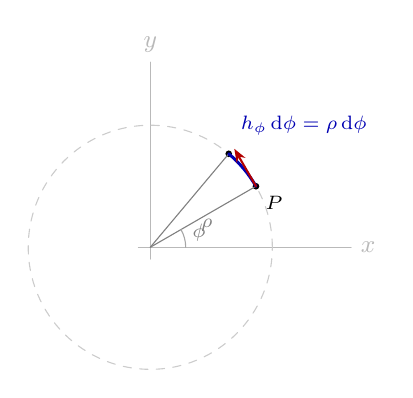
\begin{tikzpicture}[font=\small, >=Stealth, line cap=round]
  \draw[gray!55, thin] (-0.15,0) -- (2.55,0) node[right] {$x$};
  \draw[gray!55, thin] (0,-0.15) -- (0,2.35) node[above] {$y$};
  \draw[gray!40, dashed] (0,0) circle (1.55);
  \coordinate (A) at ({1.55*0.866},{1.55*0.5});
  \coordinate (B) at ({1.55*0.643},{1.55*0.766});
  \fill (A) circle (1.2pt);
  \fill (B) circle (1.2pt);
  \draw[gray] (0,0) -- (A);
  \draw[gray] (0,0) -- (B);
  \draw[blue!70!black, line width=1.1pt]
    (A) arc (30:50:1.55);
  \draw[red!70!black, -{Stealth[length=1.7mm]}, line width=0.75pt]
    (A) -- ++({0.55*(-0.5)},{0.55*0.866});
  \node[blue!70!black, font=\scriptsize] at (1.95,1.55) {$h_\phi\,\mathrm{d}\phi=\rho\,\mathrm{d}\phi$};
  \node[font=\scriptsize, gray] at (0.72,0.28) {$\rho$};
  \draw[gray!70] (0.45,0) arc (0:30:0.45);
  \node[gray, font=\scriptsize] at (0.62,0.18) {$\phi$};
  \node[font=\scriptsize] at (A) [below right] {$P$};
\end{tikzpicture}
}
    \end{column}
  \end{columns}
\end{frame}

\begin{frame}{单位矢量：沿坐标线的 $\mathrm{d}\br/\mathrm{d}s$}
  沿第 $i$ 条坐标线走，$\mathrm{d}\br=(\partial\br/\partial q_i)\,\mathrm{d}q_i$，
  此时 $\mathrm{d}s=\mathrm{d}\ell_i=h_i\,\mathrm{d}q_i$。\textbf{单位矢量}（unit vector）就是
  \begin{equation*}
    \boxed{\displaystyle
      \ue_i
      =\frac{\mathrm{d}\br}{\mathrm{d}s}
      =\frac{1}{h_i}\frac{\partial\br}{\partial q_i}.}
  \end{equation*}
  这样 $|\ue_i|=1$；正交时还有 $\ue_i\cdot\ue_j=\delta_{ij}$。
  方向导数应按弧长算，$\partial u/\partial\ell_i$，不是 $\partial u/\partial q_i$；
  梯度里的 $1/h_i$，就是这一步换元。若不除以 $h_i$，切向量长度不对，后面公式会整段错位。
\end{frame}

% \begin{frame}{位移怎样用单位基写出}
%   长度放在 $h_i\,\mathrm{d}q_i$ 里，基矢只管方向：
%   \begin{equation*}
%     \mathrm{d}\boldsymbol{\ell}
%     =\sum_{i=1}^{3} h_i\,\mathrm{d}q_i\,\ue_i.
%   \end{equation*}
%   右手系取 $\ue_1\times\ue_2=\ue_3$（柱、球坐标常用排序满足这一点）。
%   矢量写成 $\mathbf{A}=\sum A_i\ue_i$，\textbf{物理分量}（physical component）$A_i=\mathbf{A}\cdot\ue_i$
%   才是沿单位方向的投影；不归一化时点积还带着 $h_i$。
%   \vspace{0.3em}

%   这里的 $\ue_i$ 会随位置转。算散度、旋度时，不能当成常矢量提出求导。
% \end{frame}

\begin{frame}{位置矢量}
  直角基底下，位置矢量总是分量形式
  \begin{equation*}
    \br=x\,\ue_x+y\,\ue_y+z\,\ue_z.
  \end{equation*}
  柱、球只是把 $(x,y,z)$ 换成前面定义的关系式。

  \medskip
  \textbf{柱坐标}：到 $z$ 轴的距离为 $\rho$，方位角为 $\phi$，故
  $x=\rho\cos\phi$，$y=\rho\sin\phi$，高度仍是 $z$。代入得
  \begin{equation*}
    \br=\rho\cos\phi\,\ue_x+\rho\sin\phi\,\ue_y+z\,\ue_z.
  \end{equation*}

  \medskip
  \textbf{球坐标}：到原点距离为 $r$，与 $z$ 轴夹角为 $\theta$，故
  $z=r\cos\theta$，水平投影长为 $r\sin\theta$；
  再在 $xy$ 平面用方位角 $\phi$ 分解，
  $x=r\sin\theta\cos\phi$，$y=r\sin\theta\sin\phi$。代入得
  \begin{equation*}
    \br=r\sin\theta\cos\phi\,\ue_x
    +r\sin\theta\sin\phi\,\ue_y
    +r\cos\theta\,\ue_z.
  \end{equation*}
\end{frame}

\begin{frame}{例：柱坐标——尺度因子}
  \begin{columns}[T]
    \begin{column}{0.58\textwidth}
      {\small
      如前：
      $\br=\rho\cos\phi\,\ue_x+\rho\sin\phi\,\ue_y+z\,\ue_z$。
      \begin{align*}
        \partial_\rho\br&=\cos\phi\,\ue_x+\sin\phi\,\ue_y,\\
        \partial_\phi\br&=-\rho\sin\phi\,\ue_x+\rho\cos\phi\,\ue_y,\\
        \partial_z\br&=\ue_z.
      \end{align*}
      模长给出
      $\boxed{h_{\rho}=1,\ h_{\phi}=\rho,\ h_z=1.}$}
    \end{column}
    \begin{column}{0.38\textwidth}
      \centering
      \scalebox{0.88}{\begin{tikzpicture}[
    font=\small,
    >=Stealth,
    vec/.style={-{Stealth[length=2mm]}, line width=0.7pt},
  ]
  \draw[gray!55, thin] (-0.3,0) -- (2.35,0) node[right] {$x$};
  \draw[gray!55, thin] (0,-0.3) -- (0,2.35) node[above] {$y$};
  \draw[gray!45, dashed] (0,0) circle (1.35);
  \coordinate (P) at (1.08,0.72);
  \draw[gray] (0,0) -- (P);
  \fill (P) circle (1.2pt);
  \draw[vec, blue!70!black] (P) -- ++(0.55,0.37) node[right] {$\ue_{\rho}$};
  \draw[vec, red!70!black] (P) -- ++(-0.37,0.55) node[above] {$\ue_{\phi}$};
  \draw[green!50!black, line width=0.8pt] (P) circle (0.13);
  \node[green!50!black, font=\scriptsize, below left] at (P) {$\ue_{z}$};
\end{tikzpicture}
}
    \end{column}
  \end{columns}
\end{frame}

\begin{frame}{例：柱坐标——单位矢量}
  单位矢量 $\ue_i=(1/h_i)\,\partial_{q_i}\br$：
  \begin{align*}
    \ue_{\rho}
    &=\partial_\rho\br
    =\cos\phi\,\ue_x+\sin\phi\,\ue_y,\\
    \ue_{\phi}
    &=\frac{1}{\rho}\partial_\phi\br
    =-\sin\phi\,\ue_x+\cos\phi\,\ue_y,\\
    \ue_z
    &=\partial_z\br
    =\ue_z.
  \end{align*}
  三者两两正交且右手。随 $\phi$ 转动：
  $\partial_\phi\ue_{\rho}=\ue_{\phi}$，
  $\partial_\phi\ue_{\phi}=-\ue_{\rho}$。
\end{frame}

\begin{frame}{例：球坐标——尺度因子}
  \begin{columns}[T]
    \begin{column}{0.58\textwidth}
      {\small
      如前：
      $\br=r\sin\theta\cos\phi\,\ue_x+r\sin\theta\sin\phi\,\ue_y+r\cos\theta\,\ue_z$。
      \begin{align*}
        \partial_r\br
        &=\sin\theta\cos\phi\,\ue_x+\sin\theta\sin\phi\,\ue_y+\cos\theta\,\ue_z,\\
        \partial_\theta\br
        &=r(\cos\theta\cos\phi\,\ue_x+\cos\theta\sin\phi\,\ue_y-\sin\theta\,\ue_z),\\
        \partial_\phi\br
        &=r\sin\theta(-\sin\phi\,\ue_x+\cos\phi\,\ue_y).
      \end{align*}
      $\boxed{h_r=1,\ h_{\theta}=r,\ h_{\phi}=r\sin\theta.}$}
    \end{column}
    \begin{column}{0.38\textwidth}
      \centering
      \scalebox{0.82}{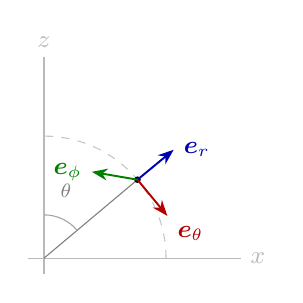
\begin{tikzpicture}[
    font=\small,
    >=Stealth,
    vec/.style={-{Stealth[length=2mm]}, line width=0.7pt},
  ]
  \draw[gray!55, thin] (-0.2,0) -- (2.5,0) node[right] {$x$};
  \draw[gray!55, thin] (0,-0.2) -- (0,2.55) node[above] {$z$};
  \draw[gray!45, dashed] (1.55,0) arc (0:90:1.55);
  \coordinate (Q) at ({1.55*0.766},{1.55*0.643});
  \draw[gray] (0,0) -- (Q);
  \fill (Q) circle (1.2pt);
  \draw[vec, blue!70!black] (Q) -- ++(0.46,0.38) node[right] {$\ue_{r}$};
  \draw[vec, red!70!black] (Q) -- ++(0.38,-0.46) node[below right] {$\ue_{\theta}$};
  \draw[vec, green!50!black] (Q) -- ++(-0.58,0.1) node[left] {$\ue_{\phi}$};
  \draw[gray!70] (0,0.55) arc (90:40:0.55);
  \node[gray, font=\scriptsize] at (0.28,0.85) {$\theta$};
\end{tikzpicture}
}
    \end{column}
  \end{columns}
\end{frame}

\begin{frame}{例：球坐标——单位矢量}
  同样 $\ue_i=(1/h_i)\,\partial_{q_i}\br$：
  \begin{align*}
    \ue_r
    &=\partial_r\br
    =\sin\theta\cos\phi\,\ue_x+\sin\theta\sin\phi\,\ue_y+\cos\theta\,\ue_z,\\
    \ue_{\theta}
    &=\frac{1}{r}\partial_\theta\br
    =\cos\theta\cos\phi\,\ue_x+\cos\theta\sin\phi\,\ue_y-\sin\theta\,\ue_z,\\
    \ue_{\phi}
    &=\frac{1}{r\sin\theta}\partial_\phi\br
    =-\sin\phi\,\ue_x+\cos\phi\,\ue_y.
  \end{align*}
  纬度圈弧长是 $r\sin\theta\,\mathrm{d}\phi$，故 $h_{\phi}$ 在两极为零；
  $\ue_r,\ue_{\theta},\ue_{\phi}$ 构成右手正交标架。
\end{frame}

\begin{frame}{面积元与体积元}
  \begin{columns}[c]
    \begin{column}{0.52\textwidth}
      三条棱长分别是 $h_i\,\mathrm{d}q_i$。正交时，
      \textbf{面积元}（area element）与\textbf{体积元}（volume element）为
      \begin{equation*}
        \mathrm{d}S_1=h_2 h_3\,\mathrm{d}q_2\,\mathrm{d}q_3,
        \quad
        \mathrm{d}V=h_1 h_2 h_3\,\mathrm{d}q_1\mathrm{d}q_2\mathrm{d}q_3.
      \end{equation*}
      $\mathrm{d}S_1$ 是法向为 $\ue_1$ 的那一面。
      把刚求出的尺度因子乘起来：
      \begin{itemize}
        \item 柱：$h_{\rho}h_{\phi}h_z=1\cdot\rho\cdot 1=\rho$，故
          $\mathrm{d}V=\rho\,\mathrm{d}\rho\,\mathrm{d}\phi\,\mathrm{d}z$；
        \item 球：$h_r h_{\theta}h_{\phi}=1\cdot r\cdot r\sin\theta=r^2\sin\theta$，故
          $\mathrm{d}V=r^2\sin\theta\,\mathrm{d}r\,\mathrm{d}\theta\,\mathrm{d}\phi$。
      \end{itemize}
    \end{column}
    \begin{column}{0.44\textwidth}
      \centering
      \scalebox{0.85}{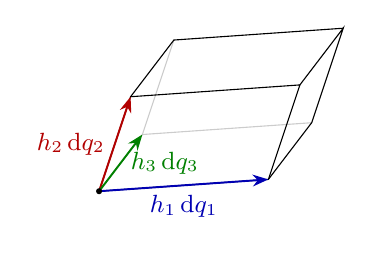
\begin{tikzpicture}[font=\small, >=Stealth, line cap=round,
    vec/.style={-{Stealth[length=2mm]}, line width=0.7pt}]
  \coordinate (O) at (0,0);
  \coordinate (A) at (2.15,0.15);
  \coordinate (B) at (2.55,1.35);
  \coordinate (C) at (0.4,1.2);
  \coordinate (D) at (0.55,0.72);
  \coordinate (E) at (2.7,0.87);
  \coordinate (F) at (3.1,2.07);
  \coordinate (G) at (0.95,1.92);
  \draw[gray!40] (O) -- (D) -- (G);
  \draw[gray!40] (D) -- (E);
  \draw (O) -- (A) -- (B) -- (C) -- cycle;
  \draw (A) -- (E) -- (F) -- (B);
  \draw (C) -- (G) -- (F);
  \draw[vec, blue!70!black] (O) -- (A) node[midway, below] {$h_1\,\mathrm{d}q_1$};
  \draw[vec, red!70!black] (O) -- (C) node[midway, left] {$h_2\,\mathrm{d}q_2$};
  \draw[vec, green!50!black] (O) -- (D) node[midway, right] {$h_3\,\mathrm{d}q_3$};
  \fill (O) circle (1.1pt);
\end{tikzpicture}
}
    \end{column}
  \end{columns}
\end{frame}

\begin{frame}{例：柱坐标——核对正交}
  \begin{align*}
    \partial_\rho\br\cdot\partial_\phi\br
    &=(\cos\phi)(-\rho\sin\phi)+(\sin\phi)(\rho\cos\phi)
     =0,\\
    \partial_\rho\br\cdot\partial_z\br
    &=(\cos\phi\,\ue_x+\sin\phi\,\ue_y)\cdot\ue_z
     =0,\\
    \partial_\phi\br\cdot\partial_z\br
    &=(-\rho\sin\phi\,\ue_x+\rho\cos\phi\,\ue_y)\cdot\ue_z
     =0.
  \end{align*}
  三对切向量两两正交，故
  \begin{equation*}
    \mathrm{d}s^2=\mathrm{d}\rho^2+\rho^2\,\mathrm{d}\phi^2+\mathrm{d}z^2.
  \end{equation*}
\end{frame}

\begin{frame}{例：椭球坐标（长旋转）}
  \begin{columns}[c]
    \begin{column}{0.50\textwidth}
      {\small
      \textbf{长旋转椭球坐标}（prolate spheroidal coordinates）$(\xi,\eta,\phi)$：
      \begin{align*}
        x&=a\sqrt{(\xi^2-1)(1-\eta^2)}\cos\phi,\\
        y&=a\sqrt{(\xi^2-1)(1-\eta^2)}\sin\phi,\\
        z&=a\xi\eta,
      \end{align*}
      其中 $\xi\geq 1$，$-1\leq\eta\leq 1$，$0\leq\phi<2\pi$，$a>0$ 是焦距参数。

      坐标面：$\xi=\mathrm{const}$ 为长旋转椭球面，
      $\eta=\mathrm{const}$ 为双叶双曲面，$\phi=\mathrm{const}$ 为子午面。
      三族彼此正交。}
    \end{column}
    \begin{column}{0.48\textwidth}
      \centering
      \resizebox{\linewidth}{!}{\begin{tikzpicture}[font=\scriptsize, >=Stealth, line cap=round,
    scale=0.95]
  % Meridian (xz): prolate spheroidal — foci on z, ellipse elongated along z
  \draw[gray!50, thin] (-1.95,0) -- (1.95,0) node[right] {$x$};
  \draw[gray!50, thin] (0,-2.15) -- (0,2.25) node[above] {$z$};
  % foci on z-axis
  \fill (0,1.05) circle (1.1pt) node[right] {$F$};
  \fill (0,-1.05) circle (1.1pt) node[right] {$F'$};
  % ξ=const: ellipse, semi-axes (b,c)=(1.35,1.75), c>b so elongated along z
  \draw[blue!70!black, thick] (0,0) ellipse (1.35 and 1.75);
  \node[blue!70!black] at (1.05,1.35) {$\xi=\mathrm{const}$};
  % η=const: east-west hyperbola, foci at (0,±1.05)
  % (x/a)^2 - (z/b)^2 = 1 with a=0.70, asymptote-ish; keep inside frame
  \draw[red!65!black, thick]
    plot[domain=0.70:1.55, samples=32]
      ({\x}, {1.05/0.70*sqrt((\x)^2-0.70^2)});
  \draw[red!65!black, thick]
    plot[domain=0.70:1.55, samples=32]
      ({\x}, {-1.05/0.70*sqrt((\x)^2-0.70^2)});
  \draw[red!65!black, thick]
    plot[domain=0.70:1.55, samples=32]
      ({-\x}, {1.05/0.70*sqrt((\x)^2-0.70^2)});
  \draw[red!65!black, thick]
    plot[domain=0.70:1.55, samples=32]
      ({-\x}, {-1.05/0.70*sqrt((\x)^2-0.70^2)});
  \node[red!65!black] at (1.55,0.55) {$\eta=\mathrm{const}$};
  \node[gray] at (0,-2.35) {子午面示意（绕 $z$ 轴旋转）};
\end{tikzpicture}
}
    \end{column}
  \end{columns}
\end{frame}

\begin{frame}{例：椭球坐标的尺度因子}
  与柱、球相同：先算 $\partial\br/\partial\xi$ 等，再取模。结果是
  \begin{equation*}
    \boxed{\displaystyle
      h_{\xi}=a\sqrt{\frac{\xi^2-\eta^2}{\xi^2-1}},
      \quad
      h_{\eta}=a\sqrt{\frac{\xi^2-\eta^2}{1-\eta^2}},
      \quad
      h_{\phi}=a\sqrt{(\xi^2-1)(1-\eta^2)}.
    }
  \end{equation*}
  体积元 $\mathrm{d}V=h_{\xi}h_{\eta}h_{\phi}\,\mathrm{d}\xi\,\mathrm{d}\eta\,\mathrm{d}\phi$。
  \vspace{0.3em}

  要点：一般公式不改，只换 $h_i$。扁旋转椭球、共焦椭球坐标同样处理；
  边界是椭球面时，就把 $\xi=\mathrm{const}$ 当作边界。
\end{frame}

\subsection{梯度}

\begin{frame}{从全微分到梯度}
  标量场沿位移的变化定义为
  \begin{equation*}
    \mathrm{d}u=\nabla u\cdot\mathrm{d}\boldsymbol{\ell}.
  \end{equation*}
  正交曲线坐标中
  $\mathrm{d}\boldsymbol{\ell}=\sum_i h_i\,\mathrm{d}q_i\,\ue_i$。
  把\textbf{梯度}（gradient）也按同一组基展开，$\nabla u=\sum_i f_i\ue_i$，则
  \begin{equation*}
    \mathrm{d}u
    =\sum_i f_i\,h_i\,\mathrm{d}q_i.
  \end{equation*}
  另一方面，把 $u$ 看成 $(q_1,q_2,q_3)$ 的函数，
  $\mathrm{d}u=\sum_i(\partial u/\partial q_i)\,\mathrm{d}q_i$。
  比较系数：
  \begin{equation*}
    f_i h_i=\frac{\partial u}{\partial q_i}
    \quad\Rightarrow\quad
    f_i=\frac{1}{h_i}\frac{\partial u}{\partial q_i}.
  \end{equation*}
\end{frame}

\begin{frame}{正交曲线坐标中的梯度}
  \begin{equation*}
    \boxed{\displaystyle
      \nabla u
      =\sum_{i=1}^{3}\frac{1}{h_i}\frac{\partial u}{\partial q_i}\,\ue_i.}
  \end{equation*}
  直角坐标 $h_i=1$ 时，回到
  $\nabla u=\partial_x u\,\ue_x+\partial_y u\,\ue_y+\partial_z u\,\ue_z$。
  \vspace{0.3em}

  热方程 $u_t=\kappa\nabla^2 u$、势方程 $\nabla^2 u=0$ 里的 $\nabla^2$，以及电场 $\mathbf{E}=-\nabla V$，都从这里出发。
\end{frame}

\begin{frame}{最陡上升与等值面}
  \begin{columns}[c]
    \begin{column}{0.48\textwidth}
      $\mathrm{d}u=|\nabla u|\,|\mathrm{d}\boldsymbol{\ell}|\cos\theta$。
      步长固定时，$\cos\theta=1$ 使 $\mathrm{d}u$ 最大，所以 $\nabla u$ 指向 $u$ 增加最快的方向。
      \vspace{0.3em}

      \textbf{等值面}（level surface）$u=\textrm{常数}$ 上 $\mathrm{d}u=0$，故梯度垂直于等值面。
    \end{column}
    \begin{column}{0.48\textwidth}
      \centering
      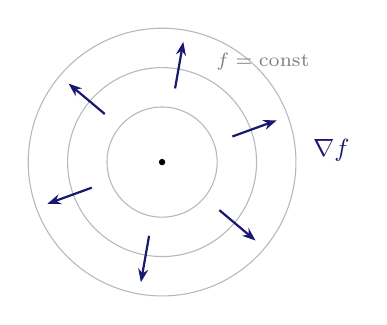
\begin{tikzpicture}[
    font=\small,
    >=Stealth,
    vec/.style={-{Stealth[length=1.7mm]}, line width=0.8pt},
  ]
  % Level sets of f=x^2+y^2 (circles) with radial gradient arrows.
  \foreach \r in {0.70,1.20,1.70} {
    \draw[gray!55] (0,0) circle (\r);
  }
  \node[gray, font=\scriptsize] at (1.28,1.28) {$f=\mathrm{const}$};

  \foreach \ang in {20,80,140,200,260,320} {
    \draw[vec, MidnightBlue]
      ({\ang}:0.95) -- ({\ang}:1.55);
  }
  \fill (0,0) circle (1.15pt);
  \node[MidnightBlue] at (2.15,0.15) {$\nabla f$};
\end{tikzpicture}

    \end{column}
  \end{columns}
\end{frame}

\begin{frame}{柱坐标梯度}
  \begin{columns}[c]
    \begin{column}{0.56\textwidth}
      $h_{\rho}=1$，$h_{\phi}=\rho$，$h_z=1$：
      \begin{equation*}
        \nabla u
        =\frac{\partial u}{\partial\rho}\,\ue_{\rho}
          +\frac{1}{\rho}\frac{\partial u}{\partial\phi}\,\ue_{\phi}
          +\frac{\partial u}{\partial z}\,\ue_z.
      \end{equation*}
      角分量里的 $1/\rho$ 就是 $1/h_{\phi}$。漏掉它，量纲就不对。
    \end{column}
    \begin{column}{0.40\textwidth}
      \centering
      \scalebox{0.85}{\begin{tikzpicture}[
    font=\small,
    >=Stealth,
    vec/.style={-{Stealth[length=2mm]}, line width=0.7pt},
  ]
  \draw[gray!55, thin] (-0.3,0) -- (2.35,0) node[right] {$x$};
  \draw[gray!55, thin] (0,-0.3) -- (0,2.35) node[above] {$y$};
  \draw[gray!45, dashed] (0,0) circle (1.35);
  \coordinate (P) at (1.08,0.72);
  \draw[gray] (0,0) -- (P);
  \fill (P) circle (1.2pt);
  \draw[vec, blue!70!black] (P) -- ++(0.55,0.37) node[right] {$\ue_{\rho}$};
  \draw[vec, red!70!black] (P) -- ++(-0.37,0.55) node[above] {$\ue_{\phi}$};
  \draw[green!50!black, line width=0.8pt] (P) circle (0.13);
  \node[green!50!black, font=\scriptsize, below left] at (P) {$\ue_{z}$};
\end{tikzpicture}
}
    \end{column}
  \end{columns}
\end{frame}

\begin{frame}{球坐标梯度}
  \begin{columns}[c]
    \begin{column}{0.56\textwidth}
      $h_r=1$，$h_{\theta}=r$，$h_{\phi}=r\sin\theta$：
      \begin{equation*}
        \nabla u
        =\frac{\partial u}{\partial r}\,\ue_r
          +\frac{1}{r}\frac{\partial u}{\partial\theta}\,\ue_{\theta}
          +\frac{1}{r\sin\theta}\frac{\partial u}{\partial\phi}\,\ue_{\phi}.
      \end{equation*}
      % 圆、球边界上的问题用这一条，不要硬套直角坐标的三项偏导。
    \end{column}
    \begin{column}{0.40\textwidth}
      \centering
      \scalebox{0.82}{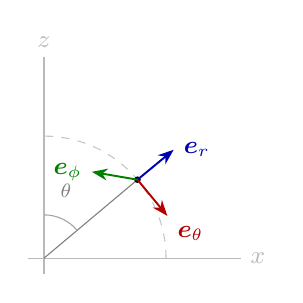
\begin{tikzpicture}[
    font=\small,
    >=Stealth,
    vec/.style={-{Stealth[length=2mm]}, line width=0.7pt},
  ]
  \draw[gray!55, thin] (-0.2,0) -- (2.5,0) node[right] {$x$};
  \draw[gray!55, thin] (0,-0.2) -- (0,2.55) node[above] {$z$};
  \draw[gray!45, dashed] (1.55,0) arc (0:90:1.55);
  \coordinate (Q) at ({1.55*0.766},{1.55*0.643});
  \draw[gray] (0,0) -- (Q);
  \fill (Q) circle (1.2pt);
  \draw[vec, blue!70!black] (Q) -- ++(0.46,0.38) node[right] {$\ue_{r}$};
  \draw[vec, red!70!black] (Q) -- ++(0.38,-0.46) node[below right] {$\ue_{\theta}$};
  \draw[vec, green!50!black] (Q) -- ++(-0.58,0.1) node[left] {$\ue_{\phi}$};
  \draw[gray!70] (0,0.55) arc (90:40:0.55);
  \node[gray, font=\scriptsize] at (0.28,0.85) {$\theta$};
\end{tikzpicture}
}
    \end{column}
  \end{columns}
\end{frame}

\begin{frame}{例}
  $u$ 只依赖 $\rho$，故 $\partial_\phi u=\partial_z u=0$。柱坐标梯度只剩第一项：
  \begin{align*}
    \nabla(\rho^2)
    &=\frac{\partial}{\partial\rho}(\rho^2)\,\ue_{\rho}
     =2\rho\,\ue_{\rho},\\
    \nabla\ln\rho
    &=\frac{\partial}{\partial\rho}(\ln\rho)\,\ue_{\rho}
     =\frac{1}{\rho}\,\ue_{\rho}
     \quad(\rho>0).
  \end{align*}
  第二式长度是 $1/\rho$，径向向外，形状和二维点源电场一样。后面算 $\nabla\cdot\mathbf{E}$ 还会用到它。
\end{frame}

\begin{frame}{梯度场的线积分只看端点}
  \begin{columns}[c]
    \begin{column}{0.52\textwidth}
      若 $\mathbf{F}=\nabla u$，则 $\nabla u\cdot\mathrm{d}\boldsymbol{\ell}=\mathrm{d}u$，于是
      \begin{equation*}
        \int_A^B\nabla u\cdot\mathrm{d}\boldsymbol{\ell}
        =u(B)-u(A).
      \end{equation*}
      闭路上 $A=B$，积分是零。保守场 $\mathbf{E}=-\nabla V$ 的环量为零，就是这一条。
    \end{column}
    \begin{column}{0.44\textwidth}
      \centering
      \scalebox{0.88}{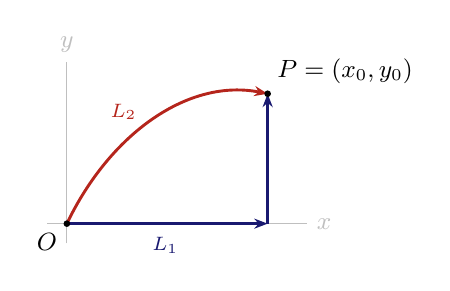
\begin{tikzpicture}[
    font=\small,
    >=Stealth,
    vec/.style={-{Stealth[length=1.8mm]}, line width=0.8pt},
  ]
  \coordinate (O) at (0,0);
  \coordinate (P) at (2.55,1.65);
  \coordinate (X) at (2.55,0);
  \coordinate (Y) at (0,1.65);

  \draw[gray!50, thin] (-0.25,0) -- (3.05,0) node[right] {$x$};
  \draw[gray!50, thin] (0,-0.25) -- (0,2.05) node[above] {$y$};

  % path 1: along axes
  \draw[MidnightBlue, line width=1.05pt, -{Stealth[length=1.7mm]}]
    (O) -- (X);
  \draw[MidnightBlue, line width=1.05pt, -{Stealth[length=1.7mm]}]
    (X) -- (P);
  \node[MidnightBlue, font=\scriptsize] at (1.25,-0.28) {$L_1$};

  % path 2: a smooth curve
  \draw[BrickRed, line width=1.05pt, -{Stealth[length=1.7mm]}]
    (O) .. controls (0.55,1.15) and (1.55,1.85) .. (P);
  \node[BrickRed, font=\scriptsize] at (0.72,1.42) {$L_2$};

  \fill (O) circle (1.2pt) node[below left] {$O$};
  \fill (P) circle (1.2pt) node[above right] {$P=(x_0,y_0)$};
\end{tikzpicture}
}
    \end{column}
  \end{columns}
\end{frame}

\begin{frame}{例：$u=x^2 y$，先算梯度}
  \begin{equation*}
    \frac{\partial u}{\partial x}=2xy,\quad
    \frac{\partial u}{\partial y}=x^2,\quad
    \frac{\partial u}{\partial z}=0,
  \end{equation*}
  故 $\nabla u=2xy\,\ue_x+x^2\,\ue_y$。
  从原点到 $P=(x_0,y_0)$，端点公式直接给出
  \begin{equation*}
    \int_O^P\nabla u\cdot\mathrm{d}\boldsymbol{\ell}
    =u(P)-u(O)=x_0^2 y_0.
  \end{equation*}
  下面用两条折线核对，确认它确实只依赖端点。
\end{frame}

\begin{frame}{例：两条折线逐步积分}
  \begin{columns}[c]
    \begin{column}{0.52\textwidth}
      {\small
      $L_1$：先沿 $x$ 轴到 $(x_0,0)$，再竖直到 $P$。\\
      第一段 $y=0$，$\mathrm{d}y=0$，被积函数 $2xy\,\mathrm{d}x=0$。\\
      第二段 $x=x_0$，$\mathrm{d}x=0$，
      $\displaystyle\int_0^{y_0}x_0^2\,\mathrm{d}y=x_0^2 y_0$。
      \vspace{0.3em}

      $L_2$：先沿 $y$ 轴到 $(0,y_0)$，再水平到 $P$。\\
      第一段 $x=0$，被积函数为零；第二段
      $\displaystyle\int_0^{x_0}2x y_0\,\mathrm{d}x=x_0^2 y_0$。
      }

      \vspace{0.35em}
      两条路径同得 $x_0^2 y_0$，与端点公式一致。
      % 但这只说明 $\nabla u$ 是保守场；
      % \textbf{拉普拉斯方程}还要另算：
      % \begin{equation*}
      %   \nabla^2 u
      %   =u_{xx}+u_{yy}+u_{zz}
      %   =2y+0+0=2y\not\equiv 0.
      % \end{equation*}
      % 故 $u=x^2 y$ \textbf{不}满足 $\nabla^2 u=0$。
      % 梯度场不必是调和函数。}
    \end{column}
    \begin{column}{0.44\textwidth}
      \centering
      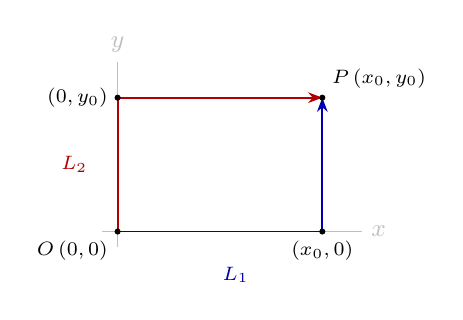
\begin{tikzpicture}[font=\small, >=Stealth,
    vec/.style={-{Stealth[length=1.8mm]}, line width=0.7pt}]
  \coordinate (O) at (0,0);
  \coordinate (P) at (2.6,1.7);
  \coordinate (X) at (2.6,0);
  \coordinate (Y) at (0,1.7);
  \draw[gray!50] (-0.2,0) -- (3.1,0) node[right] {$x$};
  \draw[gray!50] (0,-0.2) -- (0,2.15) node[above] {$y$};
  \draw[vec, blue!70!black] (O) -- (X) -- (P);
  \draw[vec, red!70!black] (O) -- (Y) -- (P);
  \fill (O) circle (1.1pt) node[below left, font=\scriptsize] {$O\,(0,0)$};
  \fill (X) circle (1.1pt) node[below, font=\scriptsize] {$(x_0,0)$};
  \fill (Y) circle (1.1pt) node[left, font=\scriptsize] {$(0,y_0)$};
  \fill (P) circle (1.1pt) node[above right, font=\scriptsize] {$P\,(x_0,y_0)$};
  \node[blue!70!black, font=\scriptsize] at (1.5,-0.55) {$L_1$};
  \node[red!70!black, font=\scriptsize] at (-0.55,0.85) {$L_2$};
\end{tikzpicture}

    \end{column}
  \end{columns}
\end{frame}

\subsection{散度}

\begin{frame}{通量与物理分量}
  闭曲面\textbf{通量}（flux）$\oint_S\mathbf{A}\cdot\mathrm{d}\mathbf{S}$，外法向。净通量为正，内部有源。
  把矢量按局部基分解，$\mathbf{A}=\sum A_i\ue_i$，其中 $A_i=\mathbf{A}\cdot\ue_i$ 是物理分量。
  \vspace{0.3em}

  \textbf{散度}（divergence）的极限定义：体积元表面净通量除以体积，
  \begin{equation*}
    \boxed{\displaystyle
      \nabla\cdot\mathbf{A}
      =\lim_{\Delta V\to 0}
        \frac{1}{\Delta V}
        \oint_{\partial(\Delta V)}\mathbf{A}\cdot\mathrm{d}\mathbf{S}.}
  \end{equation*}
  守恒律 $\rho_t+\nabla\cdot\mathbf{J}=s$ 里的 $\nabla\cdot$ 就是它。
\end{frame}

\begin{frame}{一对面的通量差：有限差分}
  \begin{columns}[T]
    \begin{column}{0.54\textwidth}
      {\small
      取 $q_1$ 方向棱长 $\Delta q_1$ 的小体元。
      法向为 $\ue_1$ 的两对面，面积元为 $h_2 h_3\,\Delta q_2\,\Delta q_3$。

      外法向通量：
      \begin{align*}
        \Phi\big|_{q_1+\Delta q_1}
        &= \bigl(A_1 h_2 h_3\bigr)\big|_{q_1+\Delta q_1}
          \,\Delta q_2\,\Delta q_3,\\
        \Phi\big|_{q_1}
        &= -\bigl(A_1 h_2 h_3\bigr)\big|_{q_1}
          \,\Delta q_2\,\Delta q_3.
      \end{align*}
      这一对的净通量（有限差分）
      \begin{equation*}
        \Delta\Phi_1
        =\Bigl[
          \bigl(A_1 h_2 h_3\bigr)\big|_{q_1+\Delta q_1}
          -\bigl(A_1 h_2 h_3\bigr)\big|_{q_1}
        \Bigr]
        \Delta q_2\,\Delta q_3.
      \end{equation*}
      除以 $\Delta q_1$ 再令 $\Delta q_1\to 0$：
      \begin{equation*}
        \Delta\Phi_1
        \to
        \frac{\partial}{\partial q_1}(A_1 h_2 h_3)\,
        \Delta q_1\,\Delta q_2\,\Delta q_3.
      \end{equation*}
      被差分的是 $A_1 h_2 h_3$，不是单独的 $A_1$。}
    \end{column}
    \begin{column}{0.42\textwidth}
      \centering
      \scalebox{0.72}{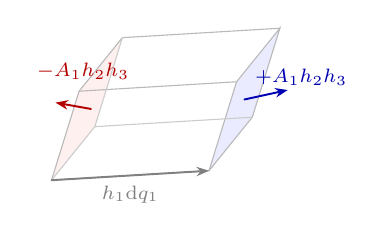
\begin{tikzpicture}[font=\scriptsize, >=Stealth, line cap=round,
    vec/.style={-{Stealth[length=1.6mm]}, line width=0.7pt}]
  \coordinate (O) at (0,0);
  \coordinate (A) at (2.0,0.12);
  \coordinate (B) at (2.35,1.25);
  \coordinate (C) at (0.35,1.13);
  \coordinate (D) at (0.55,0.68);
  \coordinate (E) at (2.55,0.80);
  \coordinate (F) at (2.90,1.93);
  \coordinate (G) at (0.90,1.81);
  \fill[blue!8] (A) -- (E) -- (F) -- (B) -- cycle;
  \fill[red!6] (O) -- (C) -- (G) -- (D) -- cycle;
  \draw[gray!55] (O) -- (A) -- (B) -- (C) -- cycle;
  \draw[gray!55] (A) -- (E) -- (F) -- (B);
  \draw[gray!55] (C) -- (G) -- (F);
  \draw[gray!40] (O) -- (D) -- (G);
  \draw[gray!40] (D) -- (E);
  \draw[vec, blue!70!black] ($(A)!0.5!(F)$) -- ++(0.55,0.12);
  \node[blue!70!black] at ($(A)!0.5!(F)+(0.72,0.28)$)
    {$+A_1 h_2 h_3$};
  \draw[vec, red!70!black] ($(O)!0.5!(G)+(0.05,0)$) -- ++(-0.45,0.08);
  \node[red!70!black] at ($(O)!0.5!(G)+(-0.05,0.48)$)
    {$-A_1 h_2 h_3$};
  \draw[vec, gray] (O) -- (A) node[midway, below] {$h_1\mathrm{d}q_1$};
\end{tikzpicture}
}
    \end{column}
  \end{columns}
\end{frame}

\begin{frame}{三个方向：同样差分，再除以体积}
  $q_2$、$q_3$ 两对面同理。记
  $H_i A_i=(h_1 h_2 h_3/h_i)A_i$（$i$ 方向的面积因子乘分量），则
  \begin{equation*}
    \Delta\Phi_i
    =\bigl[(H_i A_i)\vert_{q_i+\Delta q_i}
          -(H_i A_i)\vert_{q_i}\bigr]
    \frac{\Delta q_1\Delta q_2\Delta q_3}{\Delta q_i}.
  \end{equation*}
  令 $\Delta q_i\to 0$，三项相加得净通量
  \begin{equation*}
    \Delta\Phi
    =\sum_{i=1}^{3}
      \partial_{q_i}(H_i A_i)\,
      \Delta q_1\Delta q_2\Delta q_3.
  \end{equation*}
  除以体积 $\Delta V=h_1 h_2 h_3\,\Delta q_1\Delta q_2\Delta q_3$，得
  \begin{equation*}
    \frac{\Delta\Phi}{\Delta V}
    =\frac{1}{h_1 h_2 h_3}
      \sum_{i=1}^{3}\partial_{q_i}(H_i A_i).
  \end{equation*}
  再令体元趋于零，即
  \begin{equation*}
    \boxed{\displaystyle
      \nabla\cdot\mathbf{A}
      =\frac{1}{h_1 h_2 h_3}
        \sum_{i=1}^{3}
        \frac{\partial}{\partial q_i}
        \Bigl(\frac{h_1 h_2 h_3}{h_i} A_i\Bigr).}
  \end{equation*}
\end{frame}

\begin{frame}{直角坐标：有限差分特例}
  \begin{columns}[c]
    \begin{column}{0.52\textwidth}
      {\small
      $h_i=1$。小长方体 $\Delta x\times\Delta y\times\Delta z$：
      \begin{equation*}
        \Delta\Phi_x
        =\bigl[A_x(x+\Delta x)-A_x(x)\bigr]
        \,\Delta y\,\Delta z.
      \end{equation*}
      除以 $\Delta V=\Delta x\,\Delta y\,\Delta z$：
      \begin{equation*}
        \frac{\Delta\Phi_x}{\Delta V}
        =\frac{A_x(x+\Delta x)-A_x(x)}{\Delta x}
        \to\frac{\partial A_x}{\partial x}.
      \end{equation*}
      $y$、$z$ 同理，故
      \begin{equation*}
        \nabla\cdot\mathbf{A}
        =\partial_x A_x+\partial_y A_y+\partial_z A_z.
      \end{equation*}
      }
    \end{column}
    \begin{column}{0.44\textwidth}
      \centering
      \scalebox{0.82}{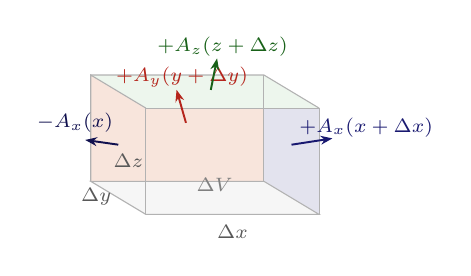
\begin{tikzpicture}[
    font=\scriptsize,
    >=Stealth,
    vec/.style={-{Stealth[length=1.5mm]}, line width=0.7pt},
  ]
  \coordinate (O) at (0,0);
  \coordinate (X) at (2.20,0);
  \coordinate (Y) at (-0.70,0.42);
  \coordinate (Z) at (0,1.35);
  \coordinate (XY) at (1.50,0.42);
  \coordinate (XZ) at (2.20,1.35);
  \coordinate (YZ) at (-0.70,1.77);
  \coordinate (XYZ) at (1.50,1.77);

  \fill[gray!7] (O) -- (X) -- (XY) -- (Y) -- cycle;
  \fill[MidnightBlue!12] (X) -- (XZ) -- (XYZ) -- (XY) -- cycle;
  \fill[BrickRed!9] (Y) -- (XY) -- (XYZ) -- (YZ) -- cycle;
  \fill[ForestGreen!8] (Z) -- (XZ) -- (XYZ) -- (YZ) -- cycle;

  \draw[gray!60] (O) -- (X) -- (XY) -- (Y) -- cycle;
  \draw[gray!60] (O) -- (Z) -- (XZ) -- (X);
  \draw[gray!60] (Z) -- (YZ) -- (Y);
  \draw[gray!60] (XZ) -- (XYZ) -- (YZ);
  \draw[gray!60] (XY) -- (XYZ);

  % edge lengths
  \node[gray!70!black] at ($(O)!0.5!(X)+(0,-0.22)$) {$\Delta x$};
  \node[gray!70!black] at ($(O)!0.5!(Y)+(-0.28,0.02)$) {$\Delta y$};
  \node[gray!70!black] at ($(O)!0.5!(Z)+(-0.22,0)$) {$\Delta z$};

  % +x face (outward)
  \coordinate (Fx) at ($(X)!0.5!(XYZ)$);
  \draw[vec, MidnightBlue] (Fx) -- ++(0.52,0.08);
  \node[MidnightBlue, align=left] at ($(Fx)+(0.95,0.22)$)
    {$+A_x(x+\Delta x)$};

  % -x face (inward contribution uses -A_x(x); arrow outward from left)
  \coordinate (Fxm) at ($(O)!0.5!(YZ)$);
  \draw[vec, MidnightBlue!70!black] (Fxm) -- ++(-0.42,0.06);
  \node[MidnightBlue!70!black, align=right] at ($(Fxm)+(-0.55,0.28)$)
    {$-A_x(x)$};

  % +y face
  \coordinate (Fy) at ($(Y)!0.55!(XYZ)$);
  \draw[vec, BrickRed] (Fy) -- ++(-0.12,0.42);
  \node[BrickRed] at ($(Fy)+(-0.05,0.58)$) {$+A_y(y+\Delta y)$};

  % +z face
  \coordinate (Fz) at ($(Z)!0.55!(XYZ)$);
  \draw[vec, ForestGreen!70!black] (Fz) -- ++(0.08,0.40);
  \node[ForestGreen!70!black] at ($(Fz)+(0.15,0.55)$) {$+A_z(z+\Delta z)$};

  \node[gray] at ($(O)!0.55!(XY)+(0.05,0.15)$) {$\Delta V$};
\end{tikzpicture}
}
    \end{column}
  \end{columns}
\end{frame}

\begin{frame}{柱坐标：把 $h_i$ 代进去}
  \begin{columns}[c]
    \begin{column}{0.56\textwidth}
      $h_{\rho}h_{\phi}h_z=\rho$。合起来
      \begin{equation*}
        \boxed{\displaystyle
          \nabla\cdot\mathbf{A}
          =\frac{1}{\rho}\frac{\partial}{\partial\rho}(\rho A_{\rho})
            +\frac{1}{\rho}\frac{\partial A_{\phi}}{\partial\phi}
            +\frac{\partial A_z}{\partial z}.}
      \end{equation*}
      第一项里的 $\rho A_{\rho}$：面积因子 $h_{\phi}h_z=\rho$ 跟着进了导数。
    \end{column}
    \begin{column}{0.40\textwidth}
      \centering
      \scalebox{0.85}{\begin{tikzpicture}[
    font=\small,
    >=Stealth,
    vec/.style={-{Stealth[length=2mm]}, line width=0.7pt},
  ]
  \draw[gray!55, thin] (-0.3,0) -- (2.35,0) node[right] {$x$};
  \draw[gray!55, thin] (0,-0.3) -- (0,2.35) node[above] {$y$};
  \draw[gray!45, dashed] (0,0) circle (1.35);
  \coordinate (P) at (1.08,0.72);
  \draw[gray] (0,0) -- (P);
  \fill (P) circle (1.2pt);
  \draw[vec, blue!70!black] (P) -- ++(0.55,0.37) node[right] {$\ue_{\rho}$};
  \draw[vec, red!70!black] (P) -- ++(-0.37,0.55) node[above] {$\ue_{\phi}$};
  \draw[green!50!black, line width=0.8pt] (P) circle (0.13);
  \node[green!50!black, font=\scriptsize, below left] at (P) {$\ue_{z}$};
\end{tikzpicture}
}
    \end{column}
  \end{columns}
\end{frame}

\begin{frame}{球坐标：把 $h_i$ 代进去}
  \begin{columns}[c]
    \begin{column}{0.60\textwidth}
      {\small
      $h_r h_{\theta}h_{\phi}=r^2\sin\theta$。
      \par\smallskip
      \resizebox{\linewidth}{!}{$\displaystyle
        \boxed{
          \nabla\cdot\mathbf{A}
          =\dfrac{1}{r^2}\partial_r(r^2 A_r)
            +\dfrac{1}{r\sin\theta}\partial_{\theta}(\sin\theta\, A_{\theta})
            +\dfrac{1}{r\sin\theta}\partial_{\phi}A_{\phi}.
        }$}
      \par\smallskip
      下面用点电荷场算一遍。}
    \end{column}
    \begin{column}{0.36\textwidth}
      \centering
      \scalebox{0.72}{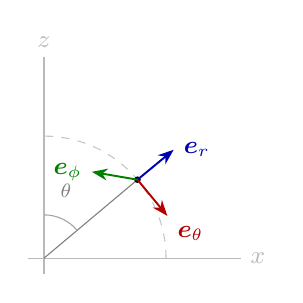
\begin{tikzpicture}[
    font=\small,
    >=Stealth,
    vec/.style={-{Stealth[length=2mm]}, line width=0.7pt},
  ]
  \draw[gray!55, thin] (-0.2,0) -- (2.5,0) node[right] {$x$};
  \draw[gray!55, thin] (0,-0.2) -- (0,2.55) node[above] {$z$};
  \draw[gray!45, dashed] (1.55,0) arc (0:90:1.55);
  \coordinate (Q) at ({1.55*0.766},{1.55*0.643});
  \draw[gray] (0,0) -- (Q);
  \fill (Q) circle (1.2pt);
  \draw[vec, blue!70!black] (Q) -- ++(0.46,0.38) node[right] {$\ue_{r}$};
  \draw[vec, red!70!black] (Q) -- ++(0.38,-0.46) node[below right] {$\ue_{\theta}$};
  \draw[vec, green!50!black] (Q) -- ++(-0.58,0.1) node[left] {$\ue_{\phi}$};
  \draw[gray!70] (0,0.55) arc (90:40:0.55);
  \node[gray, font=\scriptsize] at (0.28,0.85) {$\theta$};
\end{tikzpicture}
}
    \end{column}
  \end{columns}
\end{frame}

\begin{frame}{例：$\mathbf{A}=\ue_r/r^2$}
  \begin{columns}[T]
    \begin{column}{0.56\textwidth}
      {\small
      球坐标散度
      \par\smallskip
      \resizebox{\linewidth}{!}{$\displaystyle
        \nabla\cdot\mathbf{A}
        =\dfrac{1}{r^2}\partial_r(r^2 A_r)
          +\dfrac{1}{r\sin\theta}\partial_{\theta}(\sin\theta\, A_{\theta})
          +\dfrac{1}{r\sin\theta}\partial_{\phi}A_{\phi}.$}
      \par\smallskip
      点电荷场取 $\mathbf{A}=\ue_r/r^2$，则
      $A_r=1/r^2$，$A_{\theta}=A_{\phi}=0$，只剩第一项：
      \begin{equation*}
        \nabla\cdot\mathbf{A}
        =\frac{1}{r^2}\partial_r\bigl(r^2\cdot\tfrac{1}{r^2}\bigr)
        =\frac{1}{r^2}\partial_r(1)
        =0,
        \qquad r>0.
      \end{equation*}
      原点除外处处无源；包住原点的通量是 $4\pi$，奇性在 $r=0$。}
    \end{column}
    \begin{column}{0.40\textwidth}
      \centering
      \vspace{1.2em}
      \scalebox{0.82}{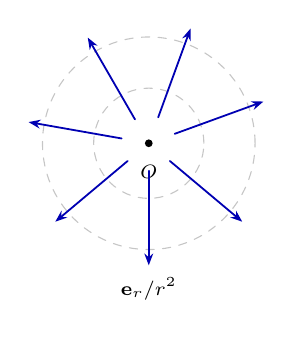
\begin{tikzpicture}[font=\small, >=Stealth, line cap=round,
    vec/.style={-{Stealth[length=1.5mm]}, line width=0.65pt}]
  \fill (0,0) circle (1.4pt);
  \node[font=\scriptsize, below] at (0,-0.15) {$O$};
  \draw[gray!45, dashed] (0,0) circle (0.7);
  \draw[gray!45, dashed] (0,0) circle (1.35);
  \foreach \ang in {20,70,120,170,220,270,320} {
    \draw[vec, blue!70!black]
      ({0.35*cos(\ang)},{0.35*sin(\ang)})
      -- ({1.55*cos(\ang)},{1.55*sin(\ang)});
  }
  \node[font=\scriptsize] at (0,-1.85) {$\mathbf{e}_r/r^2$};
\end{tikzpicture}
}
    \end{column}
  \end{columns}
\end{frame}

\begin{frame}{例：长方体上的 $\mathbf{A}=\br$}
  \small
  直角坐标散度
  $\nabla\cdot\mathbf{A}
  =\partial_x A_x+\partial_y A_y+\partial_z A_z$。
  取 $\mathbf{A}=x\ue_x+y\ue_y+z\ue_z$，则
  $\nabla\cdot\mathbf{A}
  =\partial_x x+\partial_y y+\partial_z z=3$。
  区域 $0\leq x\leq a$，$0\leq y\leq b$，$0\leq z\leq c$：
  $\int_V\nabla\cdot\mathbf{A}\,\mathrm{d}V=3abc$。
  六个面：过原点的三个面通量为零；对面 $x=a$、$y=b$、$z=c$ 各贡献 $abc$，
  合计 $\oint_S\mathbf{A}\cdot\mathrm{d}\mathbf{S}=3abc$。
  与散度定理
  $\oint_S\mathbf{A}\cdot\mathrm{d}\mathbf{S}
  =\int_V(\nabla\cdot\mathbf{A})\,\mathrm{d}V$ 两边一致。
\end{frame}

\begin{frame}{例：$\nabla\cdot\ue_{\rho}$——逐步代入}
  \begin{columns}[T]
    \begin{column}{0.54\textwidth}
      {\small
      柱坐标散度
      \begin{equation*}
        \nabla\cdot\mathbf{A}
        =\frac{1}{\rho}\partial_{\rho}(\rho A_{\rho})
          +\frac{1}{\rho}\partial_{\phi}A_{\phi}
          +\partial_z A_z.
      \end{equation*}
      取 $\mathbf{A}=\ue_{\rho}$，则 $A_{\rho}=1$，
      $A_{\phi}=A_z=0$，只留第一项：
      \begin{equation*}
        \nabla\cdot\ue_{\rho}
        =\frac{1}{\rho}\partial_{\rho}(\rho\cdot 1)
        =\frac{1}{\rho}.
      \end{equation*}
      $\ue_{\rho}$ 的方向在转，散度不是零。直角坐标里“常矢量散度为零”不能照搬到曲线基。}
    \end{column}
    \begin{column}{0.42\textwidth}
      \centering
      \vspace{1.2em}
      \scalebox{0.82}{\begin{tikzpicture}[font=\small, >=Stealth, line cap=round,
    vec/.style={-{Stealth[length=1.5mm]}, line width=0.65pt}]
  \fill (0,0) circle (1.3pt);
  \foreach \ang in {0,45,...,315} {
    \draw[vec, blue!70!black]
      ({0.45*cos(\ang)},{0.45*sin(\ang)})
      -- ({1.55*cos(\ang)},{1.55*sin(\ang)});
  }
  \draw[gray!45, dashed] (0,0) circle (1.0);
  \node[font=\scriptsize, gray] at (1.35,-0.15) {$\rho$};
  \node[font=\scriptsize] at (0,-1.95) {$\ue_{\rho}$（方向随点转动）};
\end{tikzpicture}
}
    \end{column}
  \end{columns}
\end{frame}

% \begin{frame}{与泊松方程的联系}
%   前面已得 $\nabla\cdot(\ue_r/r^2)=0$（$r\neq 0$）。
%   又 $\nabla(1/r)=-\ue_r/r^2$（$r>0$），故
%   \begin{equation*}
%     \nabla^2\Bigl(\frac{1}{r}\Bigr)
%     =\nabla\cdot\Bigl(-\frac{\ue_r}{r^2}\Bigr)
%     =0,
%     \qquad r>0.
%   \end{equation*}
%   包住原点时通量给出
%   $-\nabla^2(1/r)=4\pi\delta^3(\br)$，
%   这是\textbf{泊松方程}（Poisson equation）的基本解。
% \end{frame}

\begin{frame}{散度定理}
  由散度的定义，每个小体元 $\Delta V_\alpha$ 上
  \begin{equation*}
    \oint_{\partial(\Delta V_\alpha)}\mathbf{A}\cdot\mathrm{d}\mathbf{S}
    =(\nabla\cdot\mathbf{A})\,\Delta V_\alpha.
  \end{equation*}
  把区域 $V$ 剖成许多小体元，对 $\alpha$ 求和：
  \begin{equation*}
    \sum_\alpha
      \oint_{\partial(\Delta V_\alpha)}\mathbf{A}\cdot\mathrm{d}\mathbf{S}
    =\sum_\alpha(\nabla\cdot\mathbf{A})\,\Delta V_\alpha.
  \end{equation*}
  右边就是体积分
  $\displaystyle\int_V(\nabla\cdot\mathbf{A})\,\mathrm{d}V$。
\end{frame}

\begin{frame}{散度定理：内部面抵消}
  \begin{columns}[c]
    \begin{column}{0.50\textwidth}
      左边：相邻体元的公共面法向相反，
      $\mathbf{A}\cdot\mathrm{d}\mathbf{S}$ 成对抵消。
      \vspace{0.3em}

      留下的只有 $V$ 的外表面 $S=\partial V$。于是
      \begin{equation*}
        \sum_\alpha\oint_{\partial(\Delta V_\alpha)}
        \longrightarrow
        \oint_S\mathbf{A}\cdot\mathrm{d}\mathbf{S}.
      \end{equation*}
      这就是把局部净通量拼成整体通量的一步。
    \end{column}
    \begin{column}{0.46\textwidth}
      \centering
      \scalebox{0.82}{\begin{tikzpicture}[font=\scriptsize, >=Stealth, line cap=round,
    vec/.style={-{Stealth[length=1.2mm]}, line width=0.55pt}]
  % 4 x 3 x 3 stack of cells
  \def\dx{0.68}
  \def\dy{0.34}
  \def\dz{0.52}
  \foreach \i in {0,...,4} {
    \foreach \j in {0,...,3} {
      \foreach \k in {0,...,3} {
        \coordinate (P\i\j\k) at
          ({\i*\dx-\j*\dy},{0.40*\j*\dy+\k*\dz});
      }
    }
  }
  % bottom-layer cell fills (checker)
  \foreach \i in {0,...,3} {
    \foreach \j in {0,...,2} {
      \pgfmathtruncatemacro{\ip}{\i+1}
      \pgfmathtruncatemacro{\jp}{\j+1}
      \ifodd\numexpr\i+\j\relax
        \fill[MidnightBlue!10]
          (P\i\j0) -- (P\ip\j0) -- (P\ip\jp0) -- (P\i\jp0) -- cycle;
      \else
        \fill[MidnightBlue!5]
          (P\i\j0) -- (P\ip\j0) -- (P\ip\jp0) -- (P\i\jp0) -- cycle;
      \fi
    }
  }
  % all horizontal grids at each level
  \foreach \k in {0,...,3} {
    \foreach \j in {0,...,3} {
      \draw[gray!50, line width=0.28pt] (P0\j\k) -- (P4\j\k);
    }
    \foreach \i in {0,...,4} {
      \draw[gray!50, line width=0.28pt] (P\i0\k) -- (P\i3\k);
    }
  }
  % vertical edges
  \foreach \i in {0,...,4} {
    \foreach \j in {0,...,3} {
      \draw[gray!42, line width=0.28pt] (P\i\j0) -- (P\i\j3);
    }
  }
  % outer boundary
  \draw[MidnightBlue, line width=0.95pt]
    (P000) -- (P400) -- (P430) -- (P030) -- cycle;
  \draw[MidnightBlue, line width=0.95pt]
    (P003) -- (P403) -- (P433) -- (P033) -- cycle;
  \draw[MidnightBlue, line width=0.95pt] (P000) -- (P003);
  \draw[MidnightBlue, line width=0.95pt] (P400) -- (P403);
  \draw[MidnightBlue, line width=0.95pt] (P430) -- (P433);
  \draw[MidnightBlue, line width=0.95pt] (P030) -- (P033);
  % interior face cancellations (horizontal neighbors, mid height)
  \draw[vec, BrickRed] ($(P201)!0.2!(P211)+(0,0.10)$) -- ++(0.24,0.05);
  \draw[vec, BrickRed] ($(P201)!0.8!(P211)+(0.36,0.18)$) -- ++(-0.24,-0.05);
  \draw[vec, BrickRed] ($(P111)!0.2!(P121)+(0,0.10)$) -- ++(0.24,0.05);
  \draw[vec, BrickRed] ($(P111)!0.8!(P121)+(0.36,0.18)$) -- ++(-0.24,-0.05);
  \draw[vec, BrickRed] ($(P311)!0.2!(P321)+(0,0.10)$) -- ++(0.24,0.05);
  \draw[vec, BrickRed] ($(P311)!0.8!(P321)+(0.36,0.18)$) -- ++(-0.24,-0.05);
  % vertical neighbor cancellation
  \draw[vec, BrickRed] ($(P210)!0.35!(P211)+(-0.08,0)$) -- ++(0,0.22);
  \draw[vec, BrickRed] ($(P210)!0.35!(P211)+(0.10,0.48)$) -- ++(0,-0.22);
  \node[BrickRed] at ($(P302)!0.5!(P323)+(0.95,0.35)$) {内部面抵消};
  \node[MidnightBlue] at (1.05,-0.42) {$V=\bigcup\Delta V_\alpha$};
  \node[ForestGreen] at (3.25,2.05) {$S=\partial V$};
\end{tikzpicture}
}
    \end{column}
  \end{columns}
\end{frame}

\begin{frame}{散度定理}
  \begin{columns}[c]
    \begin{column}{0.52\textwidth}
      合起来得到\textbf{散度定理}（divergence theorem）
      \begin{equation*}
        \boxed{\displaystyle
          \oint_S\mathbf{A}\cdot\mathrm{d}\mathbf{S}
          =\int_V(\nabla\cdot\mathbf{A})\,\mathrm{d}V.}
      \end{equation*}
      外法向约定。前面长方体例子两边都是 $3abc$，就是它的特例。
      推热方程时，用它把曲面积分改成体积分。
    \end{column}
    \begin{column}{0.44\textwidth}
      \centering
      \scalebox{0.85}{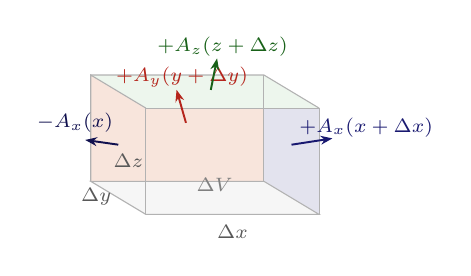
\begin{tikzpicture}[
    font=\scriptsize,
    >=Stealth,
    vec/.style={-{Stealth[length=1.5mm]}, line width=0.7pt},
  ]
  \coordinate (O) at (0,0);
  \coordinate (X) at (2.20,0);
  \coordinate (Y) at (-0.70,0.42);
  \coordinate (Z) at (0,1.35);
  \coordinate (XY) at (1.50,0.42);
  \coordinate (XZ) at (2.20,1.35);
  \coordinate (YZ) at (-0.70,1.77);
  \coordinate (XYZ) at (1.50,1.77);

  \fill[gray!7] (O) -- (X) -- (XY) -- (Y) -- cycle;
  \fill[MidnightBlue!12] (X) -- (XZ) -- (XYZ) -- (XY) -- cycle;
  \fill[BrickRed!9] (Y) -- (XY) -- (XYZ) -- (YZ) -- cycle;
  \fill[ForestGreen!8] (Z) -- (XZ) -- (XYZ) -- (YZ) -- cycle;

  \draw[gray!60] (O) -- (X) -- (XY) -- (Y) -- cycle;
  \draw[gray!60] (O) -- (Z) -- (XZ) -- (X);
  \draw[gray!60] (Z) -- (YZ) -- (Y);
  \draw[gray!60] (XZ) -- (XYZ) -- (YZ);
  \draw[gray!60] (XY) -- (XYZ);

  % edge lengths
  \node[gray!70!black] at ($(O)!0.5!(X)+(0,-0.22)$) {$\Delta x$};
  \node[gray!70!black] at ($(O)!0.5!(Y)+(-0.28,0.02)$) {$\Delta y$};
  \node[gray!70!black] at ($(O)!0.5!(Z)+(-0.22,0)$) {$\Delta z$};

  % +x face (outward)
  \coordinate (Fx) at ($(X)!0.5!(XYZ)$);
  \draw[vec, MidnightBlue] (Fx) -- ++(0.52,0.08);
  \node[MidnightBlue, align=left] at ($(Fx)+(0.95,0.22)$)
    {$+A_x(x+\Delta x)$};

  % -x face (inward contribution uses -A_x(x); arrow outward from left)
  \coordinate (Fxm) at ($(O)!0.5!(YZ)$);
  \draw[vec, MidnightBlue!70!black] (Fxm) -- ++(-0.42,0.06);
  \node[MidnightBlue!70!black, align=right] at ($(Fxm)+(-0.55,0.28)$)
    {$-A_x(x)$};

  % +y face
  \coordinate (Fy) at ($(Y)!0.55!(XYZ)$);
  \draw[vec, BrickRed] (Fy) -- ++(-0.12,0.42);
  \node[BrickRed] at ($(Fy)+(-0.05,0.58)$) {$+A_y(y+\Delta y)$};

  % +z face
  \coordinate (Fz) at ($(Z)!0.55!(XYZ)$);
  \draw[vec, ForestGreen!70!black] (Fz) -- ++(0.08,0.40);
  \node[ForestGreen!70!black] at ($(Fz)+(0.15,0.55)$) {$+A_z(z+\Delta z)$};

  \node[gray] at ($(O)!0.55!(XY)+(0.05,0.15)$) {$\Delta V$};
\end{tikzpicture}
}
    \end{column}
  \end{columns}
\end{frame}

\subsection{旋度}

\begin{frame}{环量与局部定义}
  \begin{columns}[c]
    \begin{column}{0.52\textwidth}
      闭路\textbf{环量}（circulation）$\oint_L\mathbf{A}\cdot\mathrm{d}\boldsymbol{\ell}$。
      \textbf{旋度}（curl）衡量单位面积上的环量：
      \begin{equation*}
        (\nabla\times\mathbf{A})\cdot\un
        =\lim_{\Delta S\to 0}\frac{1}{\Delta S}
          \oint_{\partial(\Delta S)}\mathbf{A}\cdot\mathrm{d}\boldsymbol{\ell}.
      \end{equation*}
      \textbf{法拉第定律}、\textbf{安培--麦克斯韦定律}里的 $\nabla\times$，用的就是这个定义。
    \end{column}
    \begin{column}{0.44\textwidth}
      \centering
      \scalebox{0.82}{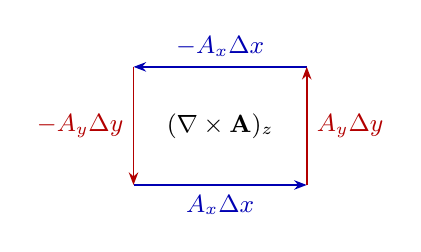
\begin{tikzpicture}[font=\small, >=Stealth,
    vec/.style={-{Stealth[length=1.6mm]}, line width=0.7pt}]
  \coordinate (O) at (0,0);
  \coordinate (X) at (2.2,0);
  \coordinate (Y) at (0,1.5);
  \coordinate (P) at (2.2,1.5);
  \draw[vec, blue!70!black] (O) -- (X) node[midway, below] {$A_x\Delta x$};
  \draw[vec, blue!70!black] (P) -- (Y) node[midway, above] {$-A_x\Delta x$};
  \draw[vec, red!70!black] (X) -- (P) node[midway, right] {$A_y\Delta y$};
  \draw[vec, red!70!black] (Y) -- (O) node[midway, left] {$-A_y\Delta y$};
  \node at (1.1,0.75) {$(\nabla\times\mathbf{A})_z$};
\end{tikzpicture}
}
    \end{column}
  \end{columns}
\end{frame}

\begin{frame}{小面片上的环量——逐步写出}
  \begin{columns}[T]
    \begin{column}{0.52\textwidth}
      {\small
      法向 $\ue_1$ 的小面片：两条 $q_2$ 边、两条 $q_3$ 边。
      切向长度 $h_2\,\mathrm{d}q_2$、$h_3\,\mathrm{d}q_3$。
      除以面积 $h_2 h_3\,\mathrm{d}q_2\,\mathrm{d}q_3$，
      \begin{equation*}
        \boxed{\displaystyle
          (\nabla\times\mathbf{A})_1
          =\frac{1}{h_2 h_3}
            \bigl(
              \partial_{q_2}(h_3 A_3)
              -\partial_{q_3}(h_2 A_2)
            \bigr).}
      \end{equation*}
      另两个分量按 $1\to 2\to 3\to 1$ 轮换。导数作用在 $h_i A_i$ 上。}
    \end{column}
    \begin{column}{0.44\textwidth}
      \centering
      \resizebox{\linewidth}{!}{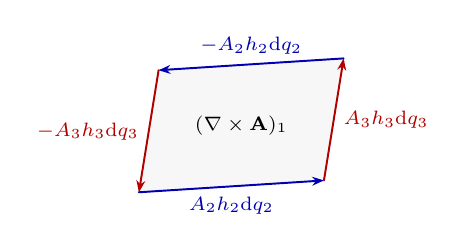
\begin{tikzpicture}[font=\scriptsize, >=Stealth, line cap=round,
    vec/.style={-{Stealth[length=1.5mm]}, line width=0.7pt}]
  \coordinate (O) at (0,0);
  \coordinate (R) at (2.35,0.15);
  \coordinate (U) at (0.25,1.55);
  \coordinate (UR) at (2.60,1.70);
  \fill[gray!6] (O) -- (R) -- (UR) -- (U) -- cycle;
  \draw[gray!60] (O) -- (R) -- (UR) -- (U) -- cycle;
  \draw[vec, blue!70!black] (O) -- (R)
    node[midway, below] {$A_2 h_2\mathrm{d}q_2$};
  \draw[vec, blue!70!black] (UR) -- (U)
    node[midway, above] {$-A_2 h_2\mathrm{d}q_2$};
  \draw[vec, red!70!black] (R) -- (UR)
    node[midway, right] {$A_3 h_3\mathrm{d}q_3$};
  \draw[vec, red!70!black] (U) -- (O)
    node[midway, left] {$-A_3 h_3\mathrm{d}q_3$};
  \node at ($(O)!0.5!(UR)$) {$(\nabla\times\mathbf{A})_1$};
\end{tikzpicture}
}
    \end{column}
  \end{columns}
\end{frame}

\begin{frame}{一般正交曲线坐标中的旋度}
  分量形式（$i,j,k$ 轮换）：
  \begin{equation*}
    (\nabla\times\mathbf{A})_i
    =\frac{1}{h_j h_k}
      \bigl(\partial_{q_j}(h_k A_k)-\partial_{q_k}(h_j A_j)\bigr).
  \end{equation*}
  合起来写成行列式（展开时对第二行求导）：
  \begin{equation*}
    \boxed{\displaystyle
      \nabla\times\mathbf{A}
      =\frac{1}{h_1 h_2 h_3}
        \begin{vmatrix}
          h_1\ue_1 & h_2\ue_2 & h_3\ue_3 \\
          \partial_{q_1} & \partial_{q_2} & \partial_{q_3} \\
          h_1 A_1 & h_2 A_2 & h_3 A_3
        \end{vmatrix}.}
  \end{equation*}
  直角坐标 $h_i=1$ 时回到
  $\nabla\times\mathbf{A}
  =\begin{vmatrix}
  \ue_x&\ue_y&\ue_z\\
  \partial_x&\partial_y&\partial_z\\
  A_x&A_y&A_z
  \end{vmatrix}$。
\end{frame}

\begin{frame}{直角坐标：四条边逐步相加}
  \begin{columns}[c]
    \begin{column}{0.50\textwidth}
      $h_i=1$，$xy$ 平面小矩形逆时针：
      \begin{align*}
        &\text{底：}A_x\Delta x,\\
        &\text{顶：}-A_x(x,y+\Delta y)\Delta x,\\
        &\text{右：}A_y(x+\Delta x)\Delta y,\\
        &\text{左：}-A_y\Delta y.
      \end{align*}
      合起来
      $\bigl(\partial_x A_y-\partial_y A_x\bigr)\Delta x\Delta y$，
      故 $(\nabla\times\mathbf{A})_z=\partial_x A_y-\partial_y A_x$。
    \end{column}
    \begin{column}{0.46\textwidth}
      \centering
      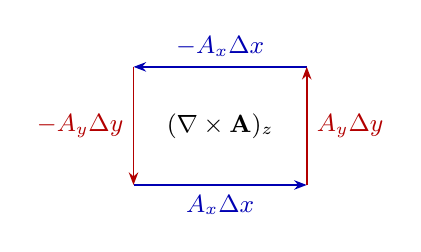
\begin{tikzpicture}[font=\small, >=Stealth,
    vec/.style={-{Stealth[length=1.6mm]}, line width=0.7pt}]
  \coordinate (O) at (0,0);
  \coordinate (X) at (2.2,0);
  \coordinate (Y) at (0,1.5);
  \coordinate (P) at (2.2,1.5);
  \draw[vec, blue!70!black] (O) -- (X) node[midway, below] {$A_x\Delta x$};
  \draw[vec, blue!70!black] (P) -- (Y) node[midway, above] {$-A_x\Delta x$};
  \draw[vec, red!70!black] (X) -- (P) node[midway, right] {$A_y\Delta y$};
  \draw[vec, red!70!black] (Y) -- (O) node[midway, left] {$-A_y\Delta y$};
  \node at (1.1,0.75) {$(\nabla\times\mathbf{A})_z$};
\end{tikzpicture}

    \end{column}
  \end{columns}
\end{frame}

\begin{frame}{柱坐标：由一般公式代入}
  一般式第 $1$ 分量
  $(\nabla\times\mathbf{A})_1
  =\frac{1}{h_2 h_3}\bigl(\partial_{q_2}(h_3 A_3)-\partial_{q_3}(h_2 A_2)\bigr)$，
  另两分量轮换。柱坐标 $h_{\rho}=1$，$h_{\phi}=\rho$，$h_z=1$，
  $(q_1,q_2,q_3)=(\rho,\phi,z)$：
  \begin{align*}
    (\nabla\times\mathbf{A})_{\rho}
    &=\frac{1}{h_{\phi}h_z}
      \bigl(\partial_{\phi}(h_z A_z)-\partial_z(h_{\phi} A_{\phi})\bigr)
    =\frac{1}{\rho}\partial_{\phi}A_z-\partial_z A_{\phi},\\
    (\nabla\times\mathbf{A})_{\phi}
    &=\frac{1}{h_z h_{\rho}}
      \bigl(\partial_z(h_{\rho} A_{\rho})-\partial_{\rho}(h_z A_z)\bigr)
    =\partial_z A_{\rho}-\partial_{\rho}A_z,\\
    (\nabla\times\mathbf{A})_z
    &=\frac{1}{h_{\rho}h_{\phi}}
      \bigl(\partial_{\rho}(h_{\phi} A_{\phi})-\partial_{\phi}(h_{\rho} A_{\rho})\bigr)
    =\frac{1}{\rho}\bigl(\partial_{\rho}(\rho A_{\phi})-\partial_{\phi}A_{\rho}\bigr).
  \end{align*}
\end{frame}

\begin{frame}{球坐标：由一般公式代入}
  球坐标 $h_r=1$，$h_{\theta}=r$，$h_{\phi}=r\sin\theta$，
  $(q_1,q_2,q_3)=(r,\theta,\phi)$。同样代入
  $(\nabla\times\mathbf{A})_i
  =\frac{1}{h_j h_k}\bigl(\partial_{q_j}(h_k A_k)-\partial_{q_k}(h_j A_j)\bigr)$：
  {\footnotesize
  \begin{align*}
    (\nabla\times\mathbf{A})_r
    &=\frac{1}{h_{\theta}h_{\phi}}
      \bigl(\partial_{\theta}(h_{\phi} A_{\phi})-\partial_{\phi}(h_{\theta} A_{\theta})\bigr)
    =\frac{1}{r\sin\theta}
      \bigl(\partial_{\theta}(\sin\theta\, A_{\phi})-\partial_{\phi}A_{\theta}\bigr),\\
    (\nabla\times\mathbf{A})_{\theta}
    &=\frac{1}{h_{\phi}h_r}
      \bigl(\partial_{\phi}(h_r A_r)-\partial_r(h_{\phi} A_{\phi})\bigr)
    =\frac{1}{r\sin\theta}\partial_{\phi}A_r
      -\frac{1}{r}\partial_r(r A_{\phi}),\\
    (\nabla\times\mathbf{A})_{\phi}
    &=\frac{1}{h_r h_{\theta}}
      \bigl(\partial_r(h_{\theta} A_{\theta})-\partial_{\theta}(h_r A_r)\bigr)
    =\frac{1}{r}\partial_r(r A_{\theta})
      -\frac{1}{r}\partial_{\theta}A_r.
  \end{align*}}
\end{frame}

\begin{frame}{斯托克斯定理：从局部定义出发}
  由旋度的局部定义，每个定向小面元 $\Delta S_\alpha$ 上
  \begin{equation*}
    \oint_{\partial(\Delta S_\alpha)}\mathbf{A}\cdot\mathrm{d}\boldsymbol{\ell}
    =(\nabla\times\mathbf{A})\cdot\un_\alpha\,\Delta S_\alpha
      +o(\Delta S_\alpha).
  \end{equation*}
  把定向曲面 $S$ 剖成许多小面元，边界定向与法向满足右手定则。
  对 $\alpha$ 求和：
  \begin{equation*}
    \sum_\alpha\oint_{\partial(\Delta S_\alpha)}\mathbf{A}\cdot\mathrm{d}\boldsymbol{\ell}
    =\sum_\alpha(\nabla\times\mathbf{A})\cdot\un_\alpha\,\Delta S_\alpha
      +o(1).
  \end{equation*}
  右边在剖分变细时就是曲面积分
  $\displaystyle\int_S(\nabla\times\mathbf{A})\cdot\mathrm{d}\mathbf{S}$。
\end{frame}

\begin{frame}{斯托克斯定理：内部边抵消}
  \begin{columns}[c]
    \begin{column}{0.50\textwidth}
      左边：相邻小面元的公共边方向相反，
      $\mathbf{A}\cdot\mathrm{d}\boldsymbol{\ell}$ 成对抵消。
      \vspace{0.3em}

      留下的只有 $S$ 的外边界 $L=\partial S$。于是
      \begin{equation*}
        \sum_\alpha\oint_{\partial(\Delta S_\alpha)}
        \longrightarrow
        \oint_L\mathbf{A}\cdot\mathrm{d}\boldsymbol{\ell}.
      \end{equation*}
      这就是把局部环量拼成整体环量的一步。
    \end{column}
    \begin{column}{0.48\textwidth}
      \centering
      \resizebox{\linewidth}{!}{\begin{tikzpicture}[font=\scriptsize, >=Stealth, line cap=round,
    vec/.style={-{Stealth[length=1.15mm]}, line width=0.55pt}]
  % denser curved surface: 5 x 3 patches (6 x 4 nodes)
  \foreach \i in {0,...,5} {
    \foreach \j in {0,...,3} {
      \coordinate (A\i\j) at
        ({0.70*\i+0.11*\j},
         {0.58*\j+0.05*\i*\i});
    }
  }
  % checker fill
  \foreach \i in {0,...,4} {
    \foreach \j in {0,...,2} {
      \pgfmathtruncatemacro{\ip}{\i+1}
      \pgfmathtruncatemacro{\jp}{\j+1}
      \ifodd\numexpr\i+\j\relax
        \fill[MidnightBlue!10]
          (A\i\j) -- (A\ip\j) -- (A\ip\jp) -- (A\i\jp) -- cycle;
      \else
        \fill[MidnightBlue!4]
          (A\i\j) -- (A\ip\j) -- (A\ip\jp) -- (A\i\jp) -- cycle;
      \fi
    }
  }
  % highlight one checker whose shared edges cancel
  \fill[BrickRed!18]
    (A21) -- (A31) -- (A32) -- (A22) -- cycle;
  % outer boundary only (no interior grey grid)
  \draw[MidnightBlue, line width=1.05pt]
    (A00) -- (A10) -- (A20) -- (A30) -- (A40) -- (A50)
          -- (A51) -- (A52) -- (A53)
          -- (A43) -- (A33) -- (A23) -- (A13) -- (A03)
          -- (A02) -- (A01) -- cycle;

  % almost-circle circulation in each patch (ccw)
  \foreach \i in {0,...,4} {
    \foreach \j in {0,...,2} {
      \pgfmathtruncatemacro{\ip}{\i+1}
      \pgfmathtruncatemacro{\jp}{\j+1}
      \path
        ($(A\i\j)!0.5!(A\ip\jp)$) coordinate (C\i\j);
      \draw[BrickRed!80!black, line width=0.55pt, -{Stealth[length=1.1mm]}]
        (C\i\j) ++(0.15,0) arc (0:320:0.15);
    }
  }

  % opposite arrows on all four edges of the highlighted checker
  % bottom A21--A31
  \draw[vec, BrickRed, line width=0.7pt]
    ($(A21)!0.20!(A31)!0.18!(A22)$) -- ($(A21)!0.80!(A31)!0.18!(A22)$);
  \draw[vec, black!70, line width=0.7pt]
    ($(A21)!0.80!(A31)!0.18!(A20)$) -- ($(A21)!0.20!(A31)!0.18!(A20)$);
  % right A31--A32
  \draw[vec, BrickRed, line width=0.7pt]
    ($(A31)!0.20!(A32)!0.18!(A21)$) -- ($(A31)!0.80!(A32)!0.18!(A21)$);
  \draw[vec, black!70, line width=0.7pt]
    ($(A31)!0.80!(A32)!0.18!(A41)$) -- ($(A31)!0.20!(A32)!0.18!(A41)$);
  % top A32--A22
  \draw[vec, BrickRed, line width=0.7pt]
    ($(A32)!0.20!(A22)!0.18!(A31)$) -- ($(A32)!0.80!(A22)!0.18!(A31)$);
  \draw[vec, black!70, line width=0.7pt]
    ($(A32)!0.80!(A22)!0.18!(A23)$) -- ($(A32)!0.20!(A22)!0.18!(A23)$);
  % left A22--A21
  \draw[vec, BrickRed, line width=0.7pt]
    ($(A22)!0.20!(A21)!0.18!(A32)$) -- ($(A22)!0.80!(A21)!0.18!(A32)$);
  \draw[vec, black!70, line width=0.7pt]
    ($(A22)!0.80!(A21)!0.18!(A12)$) -- ($(A22)!0.20!(A21)!0.18!(A12)$);

  % label completely outside, below-right
  \coordinate (Hint) at ($(A31)!0.5!(A32)$);
  \draw[BrickRed!80!black, line width=0.45pt]
    (Hint) -- ++(0.85,-0.95) coordinate (Lab);
  \node[BrickRed, anchor=north west, inner sep=1pt] at (Lab)
    {内部边抵消};

  \draw[vec, ForestGreen, line width=0.75pt]
    ($(A50)!0.12!(A53)$) -- ($(A50)!0.88!(A53)$);
  \node[ForestGreen] at ($(A50)!0.5!(A53)+(0.55,0.15)$) {$L$};
  \node[MidnightBlue] at (1.2,-0.55) {$S=\bigcup\Delta S_\alpha$};
\end{tikzpicture}
}
    \end{column}
  \end{columns}
\end{frame}

\begin{frame}{斯托克斯定理}
  \begin{columns}[c]
    \begin{column}{0.52\textwidth}
      合起来得到\textbf{斯托克斯定理}（Stokes' theorem）
      \begin{equation*}
        \boxed{\displaystyle
          \oint_L\mathbf{A}\cdot\mathrm{d}\boldsymbol{\ell}
          =\int_S(\nabla\times\mathbf{A})\cdot\mathrm{d}\mathbf{S}.}
      \end{equation*}
      环路 $L$ 与曲面法向用右手定则约定。
      张在同一条边界上的任何定向曲面，右边相同，故左边只依赖边界。
    \end{column}
    \begin{column}{0.44\textwidth}
      \centering
      \scalebox{0.82}{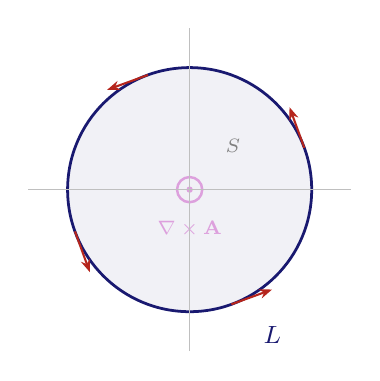
\begin{tikzpicture}[
    font=\small,
    >=Stealth,
    vec/.style={-{Stealth[length=1.6mm]}, line width=0.75pt},
  ]
  % Stokes example: circle in the xy-plane, swirl field -y e_x + x e_y.
  \def\R{1.55}
  \fill[MidnightBlue!6] (0,0) circle (\R);
  \draw[MidnightBlue, line width=1.0pt] (0,0) circle (\R);

  % tangent arrows on the circle (counterclockwise)
  \foreach \ang in {20,110,200,290} {
    \draw[vec, BrickRed]
      ({\ang}:\R) -- ++({90+\ang}:0.55);
  }

  % curl out of the page
  \draw[Plum, line width=0.9pt] (0,0) circle (0.16);
  \fill[Plum] (0,0) circle (1.15pt);
  \node[Plum, font=\scriptsize, below] at (0,-0.28) {$\nabla\times\mathbf{A}$};

  \node[MidnightBlue] at (1.05,-1.85) {$L$};
  \node[gray, font=\scriptsize] at (0.55,0.55) {$S$};
  \draw[gray!50, thin] (-2.05,0) -- (2.05,0);
  \draw[gray!50, thin] (0,-2.05) -- (0,2.05);
\end{tikzpicture}
}
    \end{column}
  \end{columns}
\end{frame}

\begin{frame}{两个基本恒等式}
  梯度没有环量，旋度没有净源：
  \begin{equation*}
    \nabla\times(\nabla u)=\mathbf{0},
    \qquad
    \nabla\cdot(\nabla\times\mathbf{A})=0.
  \end{equation*}
  所以 $\mathbf{E}=-\nabla V$ 无旋，$\mathbf{B}=\nabla\times\mathbf{A}$ 无散。
  直角分量靠混合偏导可交换就能看出来。下一节用指标再证一遍，并得到
  $\nabla\times(\nabla\times\mathbf{A})=\nabla(\nabla\cdot\mathbf{A})-\nabla^2\mathbf{A}$。
\end{frame}

\begin{frame}{例：用斯托克斯定理核对旋度}
  \footnotesize
  斯托克斯定理
  $\oint_L\mathbf{A}\cdot\mathrm{d}\boldsymbol{\ell}
  =\int_S(\nabla\times\mathbf{A})\cdot\mathrm{d}\mathbf{S}$；
  直角旋度
  $(\nabla\times\mathbf{A})_z=\partial_x A_y-\partial_y A_x$
  （另两分量轮换）。
  取 $\mathbf{A}=-y\,\ue_x+x\,\ue_y-z\,\ue_z$。
  \begin{columns}[T]
    \begin{column}{0.54\textwidth}
      $(\nabla\times\mathbf{A})_x
      =(\nabla\times\mathbf{A})_y=0$，
      $(\nabla\times\mathbf{A})_z
      =\partial_x(x)-\partial_y(-y)=2$，
      故 $\nabla\times\mathbf{A}=2\ue_z$。

      $xy$ 平面半径 $R$ 的圆
      $x=R\cos\phi$，$y=R\sin\phi$：
      $\mathbf{A}\cdot\mathrm{d}\boldsymbol{\ell}
      =-y\,\mathrm{d}x+x\,\mathrm{d}y=R^2\,\mathrm{d}\phi$，
      故 $\oint_L=2\pi R^2$。

      圆盘法向 $\ue_z$，
      $(\nabla\times\mathbf{A})\cdot\un=2$，
      故
      $\int_S(\nabla\times\mathbf{A})\cdot\mathrm{d}\mathbf{S}
      =\int_S 2\,\mathrm{d}S=2\pi R^2$，两边一致。
    \end{column}
    \begin{column}{0.42\textwidth}
      \centering
      \vspace{0.6em}
      \scalebox{0.78}{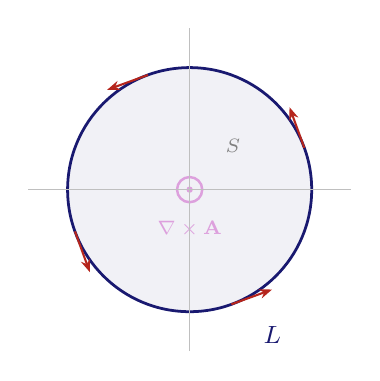
\begin{tikzpicture}[
    font=\small,
    >=Stealth,
    vec/.style={-{Stealth[length=1.6mm]}, line width=0.75pt},
  ]
  % Stokes example: circle in the xy-plane, swirl field -y e_x + x e_y.
  \def\R{1.55}
  \fill[MidnightBlue!6] (0,0) circle (\R);
  \draw[MidnightBlue, line width=1.0pt] (0,0) circle (\R);

  % tangent arrows on the circle (counterclockwise)
  \foreach \ang in {20,110,200,290} {
    \draw[vec, BrickRed]
      ({\ang}:\R) -- ++({90+\ang}:0.55);
  }

  % curl out of the page
  \draw[Plum, line width=0.9pt] (0,0) circle (0.16);
  \fill[Plum] (0,0) circle (1.15pt);
  \node[Plum, font=\scriptsize, below] at (0,-0.28) {$\nabla\times\mathbf{A}$};

  \node[MidnightBlue] at (1.05,-1.85) {$L$};
  \node[gray, font=\scriptsize] at (0.55,0.55) {$S$};
  \draw[gray!50, thin] (-2.05,0) -- (2.05,0);
  \draw[gray!50, thin] (0,-2.05) -- (0,2.05);
\end{tikzpicture}
}
    \end{column}
  \end{columns}
\end{frame}

\begin{frame}{例：直导线的磁场}
  \footnotesize
  柱坐标旋度（$h_{\rho}=1$，$h_{\phi}=\rho$，$h_z=1$）
  $(\nabla\times\mathbf{B})_z
  =\frac{1}{\rho}\bigl(\partial_{\rho}(\rho B_{\phi})-\partial_{\phi}B_{\rho}\bigr)$；
  斯托克斯
  $\oint_L\mathbf{B}\cdot\mathrm{d}\boldsymbol{\ell}
  =\int_S(\nabla\times\mathbf{B})\cdot\mathrm{d}\mathbf{S}$。
  \begin{columns}[T]
    \begin{column}{0.58\textwidth}
      无限长直导线，稳恒电流 $I$。对称性
      $\mathbf{B}=B_{\phi}(\rho)\,\ue_{\phi}$。
      \textbf{安培环路定律}
      $\oint\mathbf{B}\cdot\mathrm{d}\boldsymbol{\ell}=\mu_0 I_{\mathrm{enc}}$：
      半径 $\rho$ 的圆周上
      $2\pi\rho\, B_{\phi}=\mu_0 I$，故
      $B_{\phi}=\mu_0 I/(2\pi\rho)$（$\rho>0$）。
      （毕奥--萨伐尔同一结果。）

      此时 $B_{\rho}=0$，故
      $(\nabla\times\mathbf{B})_z
      =\frac{1}{\rho}\partial_{\rho}(\rho B_{\phi})
      =\frac{1}{\rho}\partial_{\rho}(\mu_0 I/(2\pi))
      =0$（$\rho>0$）。
      围住导线时环量仍为 $\mu_0 I$：奇性在 $\rho=0$，
      斯托克斯要求场在曲面内部光滑。
    \end{column}
    \begin{column}{0.38\textwidth}
      \centering
      \vspace{0.8em}
      \scalebox{0.82}{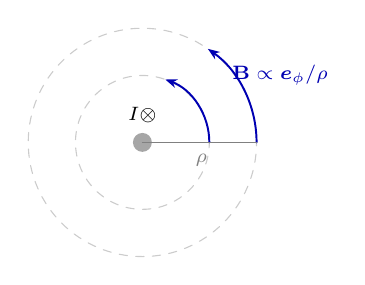
\begin{tikzpicture}[font=\small, >=Stealth, line cap=round,
    vec/.style={-{Stealth[length=1.5mm]}, line width=0.7pt}]
  \fill[gray!70] (0,0) circle (0.12);
  \node[font=\scriptsize, above] at (0,0.12) {$I\otimes$};
  \draw[gray!40, dashed] (0,0) circle (0.85);
  \draw[gray!40, dashed] (0,0) circle (1.45);
  \draw[vec, blue!70!black] (0.85,0) arc (0:70:0.85);
  \draw[vec, blue!70!black] (1.45,0) arc (0:55:1.45);
  \node[blue!70!black, font=\scriptsize] at (1.75,0.85) {$\mathbf{B}\propto\ue_{\phi}/\rho$};
  \draw[gray] (0,0) -- (1.45,0);
  \node[font=\scriptsize, gray] at (0.75,-0.22) {$\rho$};
\end{tikzpicture}
}
    \end{column}
  \end{columns}
\end{frame}

\subsection{拉普拉斯算子}

\begin{frame}{定义：$\nabla^2 u=\nabla\cdot(\nabla u)$}
  \textbf{拉普拉斯算子}（Laplacian）定义为散度作用在梯度上：
  \begin{equation*}
    \nabla^2 u=\nabla\cdot(\nabla u).
  \end{equation*}
  热方程 $u_t=\kappa\nabla^2 u$、势方程 $\nabla^2 u=0$ 或 $\nabla^2 u=f$ 用的都是它。
  推导路线：先写 $\mathbf{A}=\nabla u$ 的分量，再代入散度公式。
\end{frame}

\begin{frame}{第一步：梯度分量}
  正交曲线坐标中
  \begin{equation*}
    \nabla u
    =\sum_{i=1}^{3}
      \frac{1}{h_i}\frac{\partial u}{\partial q_i}\,\ue_i,
  \end{equation*}
  故物理分量
  \begin{equation*}
    A_i
    =(\nabla u)_i
    =\frac{1}{h_i}\frac{\partial u}{\partial q_i}.
  \end{equation*}
\end{frame}

\begin{frame}{第二步：代入散度公式}
  散度
  \begin{equation*}
    \nabla\cdot\mathbf{A}
    =\frac{1}{h_1 h_2 h_3}
      \sum_{i=1}^{3}
      \partial_{q_i}
      \Bigl(\frac{h_1 h_2 h_3}{h_i}A_i\Bigr).
  \end{equation*}
  把 $A_i=(1/h_i)\partial_{q_i}u$ 代入：
  \begin{equation*}
    \frac{h_1 h_2 h_3}{h_i}A_i
    =\frac{h_1 h_2 h_3}{h_i^2}\frac{\partial u}{\partial q_i}.
  \end{equation*}
  于是得到一般表达式
  \begin{equation*}
    \boxed{\displaystyle
      \nabla^2 u
      =\frac{1}{h_1 h_2 h_3}
        \sum_{i=1}^{3}
        \partial_{q_i}
        \Biggl(\frac{h_1 h_2 h_3}{h_i^2}\partial_{q_i}u\Biggr).}
  \end{equation*}
  不要把直角坐标的 $\partial_{xx}+\partial_{yy}+\partial_{zz}$ 换元照抄：尺度因子的导数会漏掉。
\end{frame}

\begin{frame}{柱坐标：代入尺度因子}
  \small
  一般式
  $\nabla^2 u
  =\frac{1}{h_1 h_2 h_3}
    \sum_{i=1}^{3}
    \partial_{q_i}
    \bigl((h_1 h_2 h_3/h_i^2)\partial_{q_i}u\bigr)$。
  柱坐标 $h_{\rho}=1$，$h_{\phi}=\rho$，$h_z=1$，故 $h_1 h_2 h_3=\rho$。三项：
  \begin{align*}
    i=\rho &\colon\
      \frac{1}{\rho}\partial_{\rho}(\rho\partial_{\rho}u),\\
    i=\phi &\colon\
      \frac{1}{\rho}\partial_{\phi}\bigl((\rho/\rho^2)\partial_{\phi}u\bigr)
      =\frac{1}{\rho^2}\partial_{\phi\phi}u,\\
    i=z &\colon\
      \frac{1}{\rho}\partial_z(\rho\partial_z u)
      =\partial_{zz}u.
  \end{align*}
  合起来
  \begin{equation*}
    \boxed{\displaystyle
      \nabla^2 u
      =\frac{1}{\rho}\partial_{\rho}(\rho\partial_{\rho}u)
        +\frac{1}{\rho^2}\partial_{\phi\phi}u
        +\partial_{zz}u.}
  \end{equation*}
\end{frame}

\begin{frame}{柱坐标第一项的展开}
  \begin{equation*}
    \frac{1}{\rho}\frac{\partial}{\partial\rho}
      \Bigl(\rho\frac{\partial u}{\partial\rho}\Bigr)
    =\frac{\partial^2 u}{\partial\rho^2}
      +\frac{1}{\rho}\frac{\partial u}{\partial\rho}.
  \end{equation*}
  多出来的 $(1/\rho)\partial_{\rho}u$，就是“直接换元二阶偏导”时丢掉的那一项。
  圆膜、圆柱导热的径向方程从这里来。
\end{frame}

\begin{frame}{球坐标：代入尺度因子}
  \footnotesize
  一般式
  $\nabla^2 u
  =\frac{1}{h_1 h_2 h_3}
    \sum_{i=1}^{3}
    \partial_{q_i}
    \bigl((h_1 h_2 h_3/h_i^2)\partial_{q_i}u\bigr)$。
  球坐标 $h_r=1$，$h_{\theta}=r$，$h_{\phi}=r\sin\theta$，故
  $h_1 h_2 h_3=r^2\sin\theta$。三项：
  \begin{align*}
    i=r &\colon\
      \frac{1}{r^2}\partial_r(r^2\partial_r u),\\
    i=\theta &\colon\
      \frac{1}{r^2\sin\theta}\partial_{\theta}
      (\sin\theta\,\partial_{\theta}u),\\
    i=\phi &\colon\
      \frac{1}{r^2\sin^2\theta}\partial_{\phi\phi}u.
  \end{align*}
  合起来
  \begin{equation*}
    \boxed{\displaystyle
      \nabla^2 u
      =\frac{1}{r^2}\partial_r(r^2\partial_r u)
        +\frac{1}{r^2\sin\theta}\partial_{\theta}(\sin\theta\,\partial_{\theta}u)
        +\frac{1}{r^2\sin^2\theta}\partial_{\phi\phi}u.}
  \end{equation*}
\end{frame}

\begin{frame}{例：$\nabla^2\ln\rho$——逐步计算}
  \begin{columns}[T]
    \begin{column}{0.56\textwidth}
      {\small
      柱坐标拉普拉斯
      \begin{equation*}
        \nabla^2 u
        =\frac{1}{\rho}\partial_{\rho}(\rho\partial_{\rho}u)
          +\frac{1}{\rho^2}\partial_{\phi\phi}u
          +\partial_{zz}u.
      \end{equation*}
      取 $u=\ln\rho$，则 $\partial_{\rho}u=1/\rho$，
      与 $\phi$、$z$ 无关，只留第一项：
      \begin{equation*}
        \nabla^2\ln\rho
        =\frac{1}{\rho}\partial_{\rho}
          \bigl(\rho\cdot\tfrac{1}{\rho}\bigr)
        =\frac{1}{\rho}\partial_{\rho}(1)=0,
        \qquad\rho>0.
      \end{equation*}
      若误用 $\partial_{\rho\rho}(\ln\rho)=-1/\rho^2$，结果不是零。}
    \end{column}
    \begin{column}{0.40\textwidth}
      \centering
      \vspace{1.2em}
      \scalebox{0.78}{\begin{tikzpicture}[font=\small, >=Stealth, line cap=round,
    vec/.style={-{Stealth[length=1.5mm]}, line width=0.65pt}]
  \fill (0,0) circle (1.3pt);
  \foreach \ang in {0,45,...,315} {
    \draw[vec, blue!70!black]
      ({0.45*cos(\ang)},{0.45*sin(\ang)})
      -- ({1.55*cos(\ang)},{1.55*sin(\ang)});
  }
  \draw[gray!45, dashed] (0,0) circle (1.0);
  \node[font=\scriptsize, gray] at (1.35,-0.15) {$\rho$};
  \node[font=\scriptsize] at (0,-1.95) {$\ue_{\rho}$（方向随点转动）};
\end{tikzpicture}
}
    \end{column}
  \end{columns}
\end{frame}

\begin{frame}{例：$\nabla^2(1/r)$}
  \begin{columns}[T]
    \begin{column}{0.56\textwidth}
      {\small
      球坐标拉普拉斯
      \par\smallskip
      \resizebox{\linewidth}{!}{$\displaystyle
        \nabla^2 u
        =\dfrac{1}{r^2}\partial_r(r^2\partial_r u)
          +\dfrac{1}{r^2\sin\theta}\partial_{\theta}(\sin\theta\,\partial_{\theta}u)
          +\dfrac{1}{r^2\sin^2\theta}\partial_{\phi\phi}u.$}
      \par\smallskip
      取 $u=1/r$，则 $r^2\partial_r u=-1$，与角向无关，只留第一项：
      \begin{equation*}
        \nabla^2(1/r)
        =\frac{1}{r^2}\partial_r(-1)=0,
        \qquad r>0.
      \end{equation*}
      它是球外\textbf{拉普拉斯方程}的基本解；有源时回到泊松方程。}
    \end{column}
    \begin{column}{0.40\textwidth}
      \centering
      \vspace{1.2em}
      \scalebox{0.82}{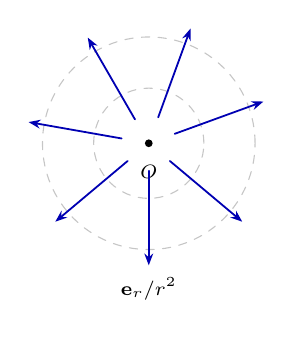
\begin{tikzpicture}[font=\small, >=Stealth, line cap=round,
    vec/.style={-{Stealth[length=1.5mm]}, line width=0.65pt}]
  \fill (0,0) circle (1.4pt);
  \node[font=\scriptsize, below] at (0,-0.15) {$O$};
  \draw[gray!45, dashed] (0,0) circle (0.7);
  \draw[gray!45, dashed] (0,0) circle (1.35);
  \foreach \ang in {20,70,120,170,220,270,320} {
    \draw[vec, blue!70!black]
      ({0.35*cos(\ang)},{0.35*sin(\ang)})
      -- ({1.55*cos(\ang)},{1.55*sin(\ang)});
  }
  \node[font=\scriptsize] at (0,-1.85) {$\mathbf{e}_r/r^2$};
\end{tikzpicture}
}
    \end{column}
  \end{columns}
\end{frame}

\begin{frame}{常用坐标：拉梅系数}
  \begin{center}
  \renewcommand{\arraystretch}{1.35}
  \begin{tabular}{lccc}
    & $h_1$ & $h_2$ & $h_3$ \\ \hline
    直角 $(x,y,z)$ & $1$ & $1$ & $1$ \\
    柱 $(\rho,\phi,z)$ & $1$ & $\rho$ & $1$ \\
    球 $(r,\theta,\phi)$ & $1$ & $r$ & $r\sin\theta$
  \end{tabular}
  \end{center}
  \vspace{0.4em}
  这张表够用了。$\nabla$、$\nabla\cdot$、$\nabla\times$、$\nabla^2$ 都是把 $h_i$ 代进一般公式。
\end{frame}

% =============================================================
\section{指标记号}

\subsection{求和约定与两个符号}

\begin{frame}{爱因斯坦求和约定}
  直角坐标里指标 $i,j,k$ 各取 $1,2,3$。\textbf{爱因斯坦求和约定}（Einstein summation convention）：同一个单项里重复出现的指标要求和，求和号不再写出。
  \begin{itemize}
    \item \textbf{哑指标}（dummy index）被求和，可以改名。
    \item \textbf{自由指标}（free index）在等式两边必须相同，并且可以改名。
  \end{itemize}
  一项之中，任何一个指标不得出现两次以上。
\end{frame}

\begin{frame}{克罗内克符号与列维--奇维塔符号}
  \textbf{克罗内克符号}（Kronecker delta）$\delta_{ij}$：$i=j$ 时为 $1$，否则为 $0$。因此 $\delta_{ii}=3$，$A_i\delta_{ij}=A_j$。
  \vspace{0.3em}

  \textbf{列维--奇维塔符号}（Levi-Civita symbol）$\varepsilon_{ijk}$：$(i,j,k)$ 是 $(1,2,3)$ 的偶置换时为 $+1$，奇置换时为 $-1$，有重复时为 $0$。
  全反对称，三个指标里有重复就为零。下面看几个直接应用。
\end{frame}

\begin{frame}{列维--奇维塔符号的应用}
  \footnotesize
  \begin{itemize}
    \item \textbf{叉积}：
      $(\mathbf{A}\times\mathbf{B})_i=\varepsilon_{ijk}A_j B_k$。
    \item \textbf{混合积}（平行六面体有向体积）：
      $\mathbf{A}\cdot(\mathbf{B}\times\mathbf{C})
      =\varepsilon_{ijk}A_i B_j C_k$。
    \item \textbf{旋度}：
      $(\nabla\times\mathbf{A})_i=\varepsilon_{ijk}\partial_j A_k$。
    \item \textbf{角动量}：
      $L_i=\varepsilon_{ijk}x_j p_k$，即 $\mathbf{L}=\mathbf{r}\times\mathbf{p}$；
      力矩同型，$M_i=\varepsilon_{ijk}x_j F_k$。
    \item \textbf{三阶行列式}：
      $\det N=\varepsilon_{ijk}N_{1i}N_{2j}N_{3k}$。
  \end{itemize}
  后面用缩并恒等式证明三重积与 $\nabla\times\nabla$、$\nabla\cdot(\nabla\times)$ 等。
\end{frame}

\begin{frame}{对称与反对称的求和规则}
  设 $S_{ij}=S_{ji}$（对称），$A_{ij}=-A_{ji}$（反对称）。则
  \begin{equation*}
    \boxed{S_{ij}A_{ij}=0.}
  \end{equation*}
  理由：把哑指标改名 $i\leftrightarrow j$，
  $S_{ij}A_{ij}=S_{ji}A_{ji}=S_{ij}(-A_{ij})=-S_{ij}A_{ij}$，
  故该项只能为零。

  \medskip
  一般规则：对某一对指标求和时，若一个因子对该对\textbf{对称}、另一个\textbf{反对称}，缩并结果为零。
  例如 $\partial_i\partial_j$ 对称、$\varepsilon_{ijk}$ 对 $(i,j)$ 反对称，故
  $\varepsilon_{ijk}\partial_i\partial_j A_k=0$，即 $\nabla\cdot(\nabla\times\mathbf{A})=0$。

  \medskip
  只保留同型部分：若 $A_{ij}$ 反对称，则
  $T_{ij}A_{ij}=T_{[ij]}A_{ij}$，其中
  $T_{[ij]}=\tfrac12(T_{ij}-T_{ji})$；对称同理用 $T_{(ij)}$。
\end{frame}

\begin{frame}{列维--奇维塔：常见等式}
  \footnotesize
  三维中常用的几条（先列出，下一页起逐条证）：
  \begin{align}
    \varepsilon_{ijk}
    &=\varepsilon_{jki}=\varepsilon_{kij}
    =-\varepsilon_{jik}=\cdots,
    \tag{E1}\\[0.2em]
    \varepsilon_{ijk}\varepsilon_{ilm}
    &=\delta_{jl}\delta_{km}-\delta_{jm}\delta_{kl},
    \tag{E2}\\[0.2em]
    \varepsilon_{ijk}\varepsilon_{ijm}
    &=2\delta_{km},
    \tag{E3}\\[0.2em]
    \varepsilon_{ijk}\varepsilon_{ijk}
    &=6,
    \tag{E4}\\[0.2em]
    \varepsilon_{ijk}\varepsilon_{klm}
    &=\delta_{il}\delta_{jm}-\delta_{im}\delta_{jl}.
    \tag{E5}
  \end{align}
  (E1) 来自定义；(E3)(E4) 由 (E2) 再缩并；(E5) 是 (E2) 改名。
\end{frame}

\begin{frame}{证 (E1)：置换符号}
  由定义：$(i,j,k)$ 是 $(1,2,3)$ 的偶置换时 $\varepsilon_{ijk}=+1$，
  奇置换时为 $-1$，有重复为 $0$。

  轮换 $(i,j,k)\mapsto(j,k,i)$ 是偶置换（两次对换），故
  $\varepsilon_{ijk}=\varepsilon_{jki}=\varepsilon_{kij}$。
  对换两个指标是奇置换，故
  $\varepsilon_{jik}=-\varepsilon_{ijk}$ 等。
\end{frame}

\begin{frame}{证 (E2)：$\varepsilon_{ijk}\varepsilon_{ilm}$}
  \footnotesize
  要证
  $\varepsilon_{ijk}\varepsilon_{ilm}
  =\delta_{jl}\delta_{km}-\delta_{jm}\delta_{kl}$。
  对指标直接核对：
  \begin{itemize}
    \item $j=k$ 或 $l=m$：左边有重复，为 $0$；右边两 $\delta$ 相减也是 $0$。
    \item $j\neq k$：对 $i$ 求和只剩与 $\{j,k\}$ 互补的那一个指标。
      若 $(l,m)=(j,k)$，两边都是 $+1$；
      若 $(l,m)=(k,j)$，两边都是 $-1$；
      若 $\{l,m\}\neq\{j,k\}$，两边都是 $0$。
  \end{itemize}
  故两边对一切取值相等。
\end{frame}

\begin{frame}{证 (E3)：$\varepsilon_{ijk}\varepsilon_{ijm}=2\delta_{km}$}
  在 (E2) 中令 $l=j$（对 $j$ 求和）：
  \begin{align*}
    \varepsilon_{ijk}\varepsilon_{ijm}
    &=\delta_{jj}\delta_{km}-\delta_{jm}\delta_{kj} \\
    &=3\,\delta_{km}-\delta_{km}
    =2\delta_{km},
  \end{align*}
  其中 $\delta_{jj}=3$，且 $\delta_{jm}\delta_{kj}=\delta_{km}$。
\end{frame}

\begin{frame}{证 (E4)：$\varepsilon_{ijk}\varepsilon_{ijk}=6$}
  在 (E3) 中令 $m=k$ 并对 $k$ 求和：
  \begin{equation*}
    \varepsilon_{ijk}\varepsilon_{ijk}
    =2\delta_{kk}
    =2\cdot 3
    =6.
  \end{equation*}
  也可直接数：$\varepsilon_{ijk}=\pm 1$ 的三元组有 $3!=6$ 个，平方和为 $6$。
\end{frame}

\begin{frame}{证 (E5)：$\varepsilon_{ijk}\varepsilon_{klm}$}
  三重积里缩并的是第三与第一指标。
  把 (E2) 中哑指标改名
  $(i,j,k,l,m)\mapsto(k,i,j,l,m)$，得到
  \begin{equation*}
    \varepsilon_{ijk}\varepsilon_{klm}
    =\delta_{il}\delta_{jm}-\delta_{im}\delta_{jl}.
  \end{equation*}
  抽查：$(i,j,l,m)=(1,2,1,2)$ 时，
  左边 $\varepsilon_{k12}\varepsilon_{k12}=\varepsilon_{312}^2=1$，
  右边 $\delta_{11}\delta_{22}-\delta_{12}\delta_{21}=1$。
\end{frame}

\begin{frame}{例：矢量三重积——第一步}
  目标：$(\mathbf{A}\times(\mathbf{B}\times\mathbf{C}))_i$。
  先写内层叉积 $(\mathbf{B}\times\mathbf{C})_k=\varepsilon_{klm}B_l C_m$，再写外层：
  \begin{equation*}
    \bigl(\mathbf{A}\times(\mathbf{B}\times\mathbf{C})\bigr)_i
    =\varepsilon_{ijk}A_j(\mathbf{B}\times\mathbf{C})_k
    =\varepsilon_{ijk}\varepsilon_{klm}A_j B_l C_m.
  \end{equation*}
  下一步用 (E5)：
  $\varepsilon_{ijk}\varepsilon_{klm}=\delta_{il}\delta_{jm}-\delta_{im}\delta_{jl}$。
\end{frame}

\begin{frame}{例：矢量三重积——完成缩并}
  \begin{align*}
    \varepsilon_{ijk}\varepsilon_{klm}A_j B_l C_m
    &=(\delta_{il}\delta_{jm}-\delta_{im}\delta_{jl})A_j B_l C_m \\
    &=A_j C_j B_i-A_j B_j C_i.
  \end{align*}
  写回矢量：
  \begin{equation*}
    \boxed{\mathbf{A}\times(\mathbf{B}\times\mathbf{C})
    =(\mathbf{A}\cdot\mathbf{C})\mathbf{B}
    -(\mathbf{A}\cdot\mathbf{B})\mathbf{C}.}
  \end{equation*}
  分解纵波与横波时常用。
\end{frame}

\begin{frame}{例：用指标算 $|\mathbf{A}\times\mathbf{B}|^2$}
  \footnotesize
  同样用叉积写法与 (E2)。
  $(\mathbf{A}\times\mathbf{B})_i=\varepsilon_{ijk}A_j B_k$，故
  \begin{align*}
    |\mathbf{A}\times\mathbf{B}|^2
    &=(\mathbf{A}\times\mathbf{B})_i(\mathbf{A}\times\mathbf{B})_i
    =\varepsilon_{ijk}\varepsilon_{ilm}A_j B_k A_l B_m \\
    &=(\delta_{jl}\delta_{km}-\delta_{jm}\delta_{kl})
      A_j B_k A_l B_m \\
    &=A_j A_j\, B_k B_k
      -A_j B_j\, A_l B_l.
  \end{align*}
  写回矢量：
  \begin{equation*}
    \boxed{|\mathbf{A}\times\mathbf{B}|^2
    =|\mathbf{A}|^2|\mathbf{B}|^2
      -(\mathbf{A}\cdot\mathbf{B})^2.}
  \end{equation*}
  右边为 $0$ 当且仅当 $\mathbf{A}\parallel\mathbf{B}$，与叉积几何意义一致。
\end{frame}

\subsection{导数恒等式}

\begin{frame}{梯度无环量}
  $(\nabla\times\nabla f)_i=\varepsilon_{ijk}\partial_j\partial_k f$。
  把哑指标 $j\leftrightarrow k$：
  \begin{equation*}
    \varepsilon_{ijk}\partial_j\partial_k f
    =\varepsilon_{ikj}\partial_k\partial_j f
    =-\varepsilon_{ijk}\partial_j\partial_k f,
  \end{equation*}
  其中用了 $\varepsilon_{ikj}=-\varepsilon_{ijk}$ 与混合偏导可交换。
  一项等于自己的相反数，故为零：
  \begin{equation*}
    \boxed{\nabla\times(\nabla f)=\mathbf{0}.}
  \end{equation*}
  所以 $\mathbf{E}=-\nabla V$ 时自动有 $\nabla\times\mathbf{E}=\mathbf{0}$。
\end{frame}

\begin{frame}{旋度无源}
  同样，
  \begin{equation*}
    \nabla\cdot(\nabla\times\mathbf{A})
    =\varepsilon_{ijk}\partial_i\partial_j A_k.
  \end{equation*}
  $\partial_i\partial_j$ 对 $(i,j)$ 对称，$\varepsilon_{ijk}$ 对 $(i,j)$ 反对称，缩并为零：
  \begin{equation*}
    \boxed{\nabla\cdot(\nabla\times\mathbf{A})=0.}
  \end{equation*}
  所以 $\mathbf{B}=\nabla\times\mathbf{A}$ 时自动有 $\nabla\cdot\mathbf{B}=0$。
\end{frame}

\begin{frame}{旋度的旋度——代入指标}
  \begin{align*}
    \bigl[\nabla\times(\nabla\times\mathbf{A})\bigr]_i
    &=\varepsilon_{ijk}\partial_j(\varepsilon_{klm}\partial_l A_m) \\
    &=\varepsilon_{ijk}\varepsilon_{klm}\,\partial_j\partial_l A_m.
  \end{align*}
  再用 (E5)
  $\varepsilon_{ijk}\varepsilon_{klm}=\delta_{il}\delta_{jm}-\delta_{im}\delta_{jl}$：
  \begin{equation*}
    (\delta_{il}\delta_{jm}-\delta_{im}\delta_{jl})\partial_j\partial_l A_m
    =\partial_i(\partial_m A_m)-\partial_j\partial_j A_i.
  \end{equation*}
\end{frame}

\begin{frame}{旋度的旋度——写回矢量}
  所以
  \begin{equation*}
    \boxed{\nabla\times(\nabla\times\mathbf{A})
    =\nabla(\nabla\cdot\mathbf{A})-\nabla^2\mathbf{A}.}
  \end{equation*}
  真空中 $\nabla\cdot\mathbf{E}=0$ 时，对法拉第和安培定律再取旋度，得到
  $\nabla^2\mathbf{E}-c^{-2}\partial_{tt}\mathbf{E}=\mathbf{0}$，主部是 $-\nabla^2$。
\end{frame}

\begin{frame}{乘积法则（指标版）}
  \begin{align*}
    \nabla\cdot(f\mathbf{A})
    &=f\,\nabla\cdot\mathbf{A}+\mathbf{A}\cdot\nabla f,\\
    \nabla\times(f\mathbf{A})
    &=f\,\nabla\times\mathbf{A}+\nabla f\times\mathbf{A},\\
    \nabla\cdot(\mathbf{A}\times\mathbf{B})
    &=\mathbf{B}\cdot(\nabla\times\mathbf{A})
      -\mathbf{A}\cdot(\nabla\times\mathbf{B}).
  \end{align*}
  同一缩并还给出
  \begin{equation*}
    \mathbf{u}\times(\nabla\times\mathbf{u})
    =\nabla\Bigl(\tfrac12|\mathbf{u}|^2\Bigr)
    -(\mathbf{u}\cdot\nabla)\mathbf{u}.
  \end{equation*}
\end{frame}

\begin{frame}{例：真空麦克斯韦方程}
  \footnotesize
  真空中的\textbf{麦克斯韦方程}（Maxwell's equations）：
  \begin{equation*}
  \begin{aligned}
    \nabla\cdot\mathbf{E}&=\rho/\varepsilon_0, &
    \nabla\cdot\mathbf{B}&=0,\\
    \nabla\times\mathbf{E}&=-\partial_t\mathbf{B}, &
    \nabla\times\mathbf{B}
    &=\mu_0\mathbf{J}+\mu_0\varepsilon_0\partial_t\mathbf{E}.
  \end{aligned}
  \end{equation*}
  对法拉第定律取散度：左边 $\nabla\cdot(\nabla\times\mathbf{E})=0$，故
  $\partial_t(\nabla\cdot\mathbf{B})=0$，与 $\nabla\cdot\mathbf{B}=0$ 相容。

  对安培--麦克斯韦定律取散度，并用 $\nabla\cdot\mathbf{E}=\rho/\varepsilon_0$，
  得连续性方程 $\partial_t\rho+\nabla\cdot\mathbf{J}=0$。

  对法拉第定律再取旋度，用
  $\nabla\times(\nabla\times\mathbf{E})=\nabla(\nabla\cdot\mathbf{E})-\nabla^2\mathbf{E}$，
  无源时 $\nabla^2\mathbf{E}-c^{-2}\partial_{tt}\mathbf{E}=\mathbf{0}$。
\end{frame}

% % =============================================================
% \section{张量}

% \subsection{阶与坐标变换}

% \begin{frame}{阶与独立分量}
%   指标的个数叫做\textbf{阶}（order / rank）。标量 $0$ 阶，矢量 $1$ 阶；$n$ 维里 $r$ 阶\textbf{张量}（tensor）在计入对称性前有 $n^r$ 个分量。
%   \vspace{0.3em}

%   对称二阶：$n(n+1)/2$ 个独立分量；反对称：$n(n-1)/2$ 个。任意二阶张量拆成
%   \begin{equation*}
%     T_{ij}
%     =\tfrac12(T_{ij}+T_{ji})
%     +\tfrac12(T_{ij}-T_{ji}).
%   \end{equation*}
%   位移梯度 $\partial_i u_j$ 的对称部分是\textbf{应变}（strain），反对称部分是无穷小转动。
% \end{frame}

% \begin{frame}{怎么判断是不是张量}
%   有一排带指标的数，不等于张量。判据是\textbf{变换律}：
%   坐标旋转 $x'_i=R_{ij}x_j$ 下，分量必须按每个指标各乘一个 $R$ 变过去，例如
%   \begin{equation*}
%     v'_i=R_{ij}v_j,
%     \qquad
%     T'_{ij}=R_{ik}R_{jl}T_{kl}.
%   \end{equation*}
%   满足这个律，换坐标系后物理关系形式不变，才叫张量。

%   \medskip
%   实用检验（商法则）：若对任意矢量 $v_j$，量 $u_i=T_{ij}v_j$ 都是矢量，则 $T_{ij}$ 是二阶张量。
% \end{frame}

% \begin{frame}{作为线性映射}
%   二阶张量把矢量送到矢量：$u_i=T_{ij}v_j$。
%   三阶张量可以吃进两个矢量：$w_i=C_{ijk}u_j v_k$。
%   \vspace{0.3em}

%   直角坐标旋转下，$\delta_{ij}$ 不变；$\varepsilon_{ijk}$ 在正常旋转下也不变，反射会多一个 $\det R=-1$。
%   后面克里斯托费尔符号 $\Gamma^{i}{}_{jk}$ 有三个指标，但变换律多出一项，故\textbf{不是}张量。
% \end{frame}

% \begin{frame}{物理中的二阶与更高阶}
%   \textbf{应力}（stress）$\sigma_{ij}$：
%   面元上的力 $\mathrm{d}F_i=\sigma_{ij}\,\mathrm{d}S_j$。
%   $\sigma_{ij}$ 表示法向沿 $j$、力沿 $i$ 的面力密度。

%   \medskip
%   \textbf{应变}（strain）$\varepsilon_{kl}$：
%   位移场的对称梯度，描写局部形变。
%   线性弹性用四阶\textbf{刚度张量}（stiffness）联结二者：
%   $\sigma_{ij}=C_{ijkl}\varepsilon_{kl}$。
%   \textbf{各向同性}（isotropic）时
%   $\sigma_{ij}=\lambda\,\delta_{ij}\varepsilon_{kk}+2\mu\,\varepsilon_{ij}$。
% \end{frame}

% \begin{frame}{电导与压电}
%   \textbf{电导率}（conductivity）$\sigma_{ij}$：
%   电场驱动电流，$J_i=\sigma_{ij}E_j$。
%   各向同性时 $\mathbf{J}=\sigma\mathbf{E}$；
%   晶体中 $\sigma_{ij}$ 可不对角，故 $\mathbf{J}$ 不必平行于 $\mathbf{E}$。

%   \medskip
%   \textbf{压电}（piezoelectricity）：
%   应力引起电极化，$P_i=d_{ijk}\sigma_{jk}$。
%   三阶张量 $d_{ijk}$ 把二阶应力映到极化矢量 $\mathbf{P}$。
% \end{frame}

% \subsection{各向同性张量}

% \begin{frame}{由 $\delta$ 与 $\varepsilon$ 拼出来}
%   旋转下形式不变的张量：
%   \begin{itemize}
%     \item $0$ 阶：常数；
%     \item $1$ 阶：只有零矢量；
%     \item $2$ 阶：$\lambda\delta_{ij}$；
%     \item $3$ 阶：$\lambda\varepsilon_{ijk}$；
%     \item $4$ 阶：
%       $T_{ijkl}=\alpha\,\delta_{ij}\delta_{kl}+\beta\,\delta_{ik}\delta_{jl}+\gamma\,\delta_{il}\delta_{jk}$。
%   \end{itemize}
%   弹性张量还要满足指标对称，所以 $\beta=\gamma$，独立常数减成两个，对应\textbf{拉梅常数}（Lamé constants）$\lambda,\mu$。
% \end{frame}

% \subsection{度规、联络与曲率}

% \begin{frame}{度规与尺度因子}
%   曲线坐标里，坐标差 $\mathrm{d}x^\mu$ 不是弧长。\textbf{度规}（metric）把弧长写成
%   \begin{equation*}
%     \mathrm{d}s^2=g_{\mu\nu}\,\mathrm{d}x^\mu\mathrm{d}x^\nu.
%   \end{equation*}
%   平面极坐标：$g_{rr}=1$，$g_{\vartheta\vartheta}=r^2$，
%   \begin{equation*}
%     h_r=\sqrt{g_{rr}}=1,
%     \qquad
%     h_{\vartheta}=\sqrt{g_{\vartheta\vartheta}}=r,
%   \end{equation*}
%   与前面尺度因子的定义一致。
% \end{frame}

% % \begin{frame}{克里斯托费尔符号}
% %   \textbf{克里斯托费尔符号}（Christoffel symbols）
% %   \begin{equation*}
% %     \Gamma^\rho{}_{\mu\nu}
% %     =\tfrac12 g^{\rho\sigma}
% %       \bigl(
% %         \partial_\mu g_{\nu\sigma}
% %         +\partial_\nu g_{\mu\sigma}
% %         -\partial_\sigma g_{\mu\nu}
% %       \bigr).
% %   \end{equation*}
% %   它描写坐标基随位置如何转动，用来写协变导数。
% %   平面极坐标非零的只有
% %   \begin{equation*}
% %     \Gamma^r{}_{\vartheta\vartheta}=-r,
% %     \qquad
% %     \Gamma^\vartheta{}_{\,r\vartheta}
% %     =\Gamma^\vartheta{}_{\,\vartheta r}=1/r.
% %   \end{equation*}
% % \end{frame}

% % \begin{frame}{为什么 $\Gamma$ 不是张量}
% %   若 $\Gamma^\rho{}_{\mu\nu}$ 是三阶张量，直角坐标里它全为零，则\textbf{一切}坐标系里都必须为零。
% %   但换到极坐标立刻出现 $\Gamma^r{}_{\vartheta\vartheta}=-r\neq 0$。
% %   所以它不满足张量变换律。

% %   \medskip
% %   一般坐标变换 $x\to x'$ 下，真正的变换式多出一项：
% %   \begin{equation*}
% %     \Gamma'^{\rho}{}_{\mu\nu}
% %     =\frac{\partial x'^{\rho}}{\partial x^{\alpha}}
% %       \frac{\partial x^{\beta}}{\partial x'^{\mu}}
% %       \frac{\partial x^{\gamma}}{\partial x'^{\nu}}
% %       \Gamma^{\alpha}{}_{\beta\gamma}
% %       +\frac{\partial x'^{\rho}}{\partial x^{\alpha}}
% %         \frac{\partial^2 x^{\alpha}}{\partial x'^{\mu}\partial x'^{\nu}}.
% %   \end{equation*}
% %   第二项含二阶导数，不是三个雅可比的齐一次式；张量不容许这种非齐次项。
% % \end{frame}

% % \begin{frame}{曲率才按张量变换}
% %   \textbf{黎曼曲率}（Riemann curvature）
% %   \begin{equation*}
% %     R^\rho{}_{\sigma\mu\nu}
% %     =\partial_\mu\Gamma^\rho{}_{\nu\sigma}
% %     -\partial_\nu\Gamma^\rho{}_{\mu\sigma}
% %     +\Gamma^\rho{}_{\mu\lambda}\Gamma^\lambda{}_{\nu\sigma}
% %     -\Gamma^\rho{}_{\nu\lambda}\Gamma^\lambda{}_{\mu\sigma}.
% %   \end{equation*}
% %   平面极坐标里 $R^r{}_{\vartheta r\vartheta}=-1+1=0$：平面的曲率张量是零，$\Gamma$ 的出现只是坐标效应。
% % \end{frame}

% \subsection{惯量张量}

% \begin{frame}{惯量张量}
%   \begin{columns}[c]
%     \begin{column}{0.52\textwidth}
%       \textbf{惯量张量}（inertia tensor）$L_i=I_{ij}\omega_j$，其中
%       \begin{equation*}
%         I_{ij}
%         =\sum_a m_a
%           \bigl(
%             |\mathbf{r}^{(a)}|^2\delta_{ij}
%             -r^{(a)}_i r^{(a)}_j
%           \bigr).
%       \end{equation*}
%       $I_{ij}=I_{ji}$。存在\textbf{主轴}（principal axes）使它对角；三个主转动惯量一般不同，故 $\mathbf{L}$ 不必平行于 $\boldsymbol{\omega}$。
%     \end{column}
%     \begin{column}{0.44\textwidth}
%       \centering
%       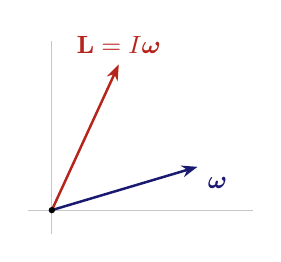
\begin{tikzpicture}[
    font=\small,
    >=Stealth,
    vec/.style={-{Stealth[length=2.0mm]}, line width=0.9pt},
  ]
  % Angular velocity and angular momentum need not be parallel.
  \draw[gray!45, thin] (-0.3,0) -- (2.55,0);
  \draw[gray!45, thin] (0,-0.3) -- (0,2.15);
  \draw[vec, MidnightBlue] (0,0) -- (1.85,0.55)
    node[below right] {$\boldsymbol{\omega}$};
  \draw[vec, BrickRed] (0,0) -- (0.85,1.85)
    node[above] {$\mathbf{L}=I\boldsymbol{\omega}$};
  \fill (0,0) circle (1.15pt);
\end{tikzpicture}

%     \end{column}
%   \end{columns}
% \end{frame}

% \begin{frame}{运算量怎么数}
%   约定：一次乘法（或乘加）算一次运算。指标每个取 $n$ 个值。

%   \medskip
%   矩阵--矢量 $w_j=B_{jk}v_k$：固定 $j$，对 $k$ 求和要 $n$ 次；
%   $j$ 有 $n$ 个，故共 $n\cdot n=n^2$。

%   \medskip
%   矩阵--矩阵 $M_{ik}=A_{ij}B_{jk}$：固定 $(i,k)$，对 $j$ 求和要 $n$ 次；
%   $(i,k)$ 有 $n^2$ 对，故共 $n^2\cdot n=n^3$。

%   \medskip
%   点积 $s=u_i z_i$：对 $i$ 求和，$n$ 次。
% \end{frame}

% \begin{frame}{缩并的次序与计算量}
%   标量 $s=u_i A_{ij}B_{jk}v_k$，结果与次序无关，运算量不同。

%   \medskip
%   \textbf{先乘矢量：}
%   $w_j=B_{jk}v_k$（$n^2$）$\to$
%   $z_i=A_{ij}w_j$（$n^2$）$\to$
%   $s=u_i z_i$（$n$），合计 $2n^2+n$。

%   \medskip
%   \textbf{先乘矩阵：}
%   $M_{ik}=A_{ij}B_{jk}$（$n^3$）$\to$
%   $y_i=M_{ik}v_k$（$n^2$）$\to$
%   $s=u_i y_i$（$n$），合计 $n^3+n^2+n$。

%   $n=10^3$ 时约为 $2\times 10^6$ 对 $10^9$。
% \end{frame}

% \begin{frame}{一般三指标缩并}
%   $A_{ij}B_{jk}C_{ki}$，设 $i\leq n$，$j\leq m$，$k\leq p$。

%   \medskip
%   先 $(BC)_{ji}=B_{jk}C_{ki}$：固定 $(j,i)$ 对 $k$ 求和，
%   运算量 $nm\cdot p=nmp$；
%   再 $A_{ij}(BC)_{ji}$：固定 $(i,j)$ 一次乘加，运算量 $nm$。
%   合计 $nmp+nm$。

%   \medskip
%   先 $(AB)_{ik}=A_{ij}B_{jk}$：运算量 $np\cdot m=nmp$；
%   再 $(AB)_{ik}C_{ki}$：运算量 $np$。
%   合计 $nmp+np$。

%   先消掉取值范围大的指标，第二步更省。
% \end{frame}

\end{document}
